\chapter{AHTR Plank Optimization Results}
\glsresetall
\label{chap:ahtr-plank-opt-results}
In this chapter, I report the \gls{AHTR} plank's \gls{ROLLO} optimization results. 
I vary the following \gls{AHTR} plank input parameters:
\begin{itemize}
    \item \gls{TRISO} packing fraction distribution ($\rho_{TRISO}(\vec{r})$)
    \item Total fuel packing fraction ($PF_{total}$)
    \item Coolant channel shape
\end{itemize} 
And, I optimize the \gls{AHTR} plank for the following optimization objectives:
\begin{itemize}
    \item Minimize total fuel packing fraction ($PF_{total}$)
    \item Minimize maximum plank temperature ($T_{max}$)
    \item Minimize fuel-normalized power peaking factor ($PPF_{fuel}$)
\end{itemize} 

In the previous chapter, I detailed the methodology for \gls{AHTR} plank modeling and 
\gls{ROLLO} optimization. 
Section \ref{sec:ahtr-plank-geometry} describes the \gls{AHTR} plank geometry.
Section \ref{sec:input-parameter-modeling} details about how I vary the 
\gls{AHTR} plank's input parameters. 
Sections \ref{sec:ahtr-moltres-hom} and \ref{sec:ahtr_model_verification}
describe and verify the \gls{AHTR} plank's OpenMC neutronics and Moltres 
temperature models. 
Section \ref{sec:opt-problem} describes the optimization objectives and Section 
\ref{sec:ahtr_slab_output} describes how I calculated them from the OpenMC and Moltres 
model outputs. 
Section \ref{sec:hyperparameter-studies} describes the hyperparameter tuning process 
to select hyperparameters for the single-objective and multi-objective \gls{ROLLO} 
optimization simulations.

The subsequent sections outline the \gls{AHTR} plank optimization simulations, describe 
the single-objective and multi-objective \gls{ROLLO} optimization simulation results, 
report each simulation's computational cost, and discuss the results' 
significance.

\section{ROLLO AHTR Plank Optimization Simulations Overview}
Table \ref{tab:slab-obj-breakdown} shows the details of each \gls{ROLLO} 
optimization simulation conducted in this chapter.
\begin{table}[htbp!]
    \centering
    \onehalfspacing
    \caption{\acrfull{ROLLO} simulations for optimizing \acrfull{AHTR}
    plank. $PF_{total}$: Total fuel packing fraction, $T_{max}$: Maximum plank temperature, 
    $PPF_{fuel}$: Fuel-normalized power peaking factor, $\rho_{TRISO}(\vec{r})$: 
    \gls{TRISO} particle distribution}
	\label{tab:slab-obj-breakdown}
    \footnotesize
    \begin{tabular}{p{1cm}|p{1cm}|llll}
    \hline 
    \textbf{Objs} & \textbf{Sim} & \textbf{Objectives} & \textbf{Constraints} &\textbf{Varying Parameters} & \textbf{Simulation Software} \\
    \hline
    \multirow{7}{2cm}{1} & p-1a & \tabitem min($PF_{total}$) & \tabitem $k_{eff}$ $\geq$ 1.35 &\tabitem $\rho_{TRISO}(\vec{r})$ & OpenMC \\
    & & & & \tabitem $PF_{total}$ & \\
    \cline{2-6}
    & p-1b & \tabitem min($T_{max}$) & \tabitem $k_{eff}$ $\geq$ 1.0 &\tabitem $\rho_{TRISO}(\vec{r})$ & OpenMC, Moltres\\
    \cline{2-6}
    & p-1c & \tabitem min($PPF_{fuel}$) & \tabitem $k_{eff}$ $\geq$ 1.0 &\tabitem $\rho_{TRISO}(\vec{r})$ & OpenMC\\
    \cline{2-6}
    & p-1d & \tabitem min($PF_{total}$) & \tabitem $k_{eff}$ $\geq$ 1.35 &\tabitem Coolant channel shape & OpenMC \\
    & & & & \tabitem $PF_{total}$ & \\
    \cline{2-6}
    & p-1e & \tabitem min($T_{max}$) & \tabitem $k_{eff}$ $\geq$ 1.35 &\tabitem Coolant channel shape & OpenMC, Moltres\\
    \cline{2-6}
    & p-1f & \tabitem min($PPF_{fuel}$) & \tabitem $k_{eff}$ $\geq$ 1.35 &\tabitem Coolant channel shape & OpenMC\\
    \hline
    \multirow{6}{2cm}{2}& p-2a & \tabitem min($PF_{total}$) & \tabitem $k_{eff}$ $\geq$ 1.35 & \tabitem $\rho_{TRISO}(\vec{r})$ & OpenMC, Moltres\\
    & &\tabitem min($T_{max}$) & & \tabitem $PF_{total}$ & \\
    \cline{2-6}
    & p-2b & \tabitem min($PF_{total}$) & \tabitem $k_{eff}$ $\geq$ 1.35 & \tabitem $\rho_{TRISO}(\vec{r})$ & OpenMC\\
    & & \tabitem min($PPF_{fuel}$) & & \tabitem $PF_{total}$ & \\
    \cline{2-6}
    & p-2c & \tabitem min($T_{max}$) & \tabitem $k_{eff}$ $\geq$ 1.0 & \tabitem $\rho_{TRISO}(\vec{r})$ & OpenMC, Moltres\\
    & & \tabitem min($PPF_{fuel}$) & & & \\
    \hline
    \multirow{6}{2cm}{3}& p-3a &\tabitem min($PF_{total}$) & \tabitem $k_{eff}$ $\geq$ 1.35 & \tabitem $\rho_{TRISO}(\vec{r})$ & OpenMC, Moltres\\
    && \tabitem min($PPF_{fuel}$) & & \tabitem $PF_{total}$ & \\
    && \tabitem min($T_{max}$) & & & \\
    \cline{2-6}
    & p-3b &\tabitem min($PF_{total}$) & \tabitem $k_{eff}$ $\geq$ 1.35 & \tabitem $\rho_{TRISO}(\vec{r})$ & OpenMC, Moltres\\
    && \tabitem min($PPF_{fuel}$) & & \tabitem $PF_{total}$ & \\
    && \tabitem min($T_{max}$) & & \tabitem Coolant channel shape& \\
    \hline
    \end{tabular}
\end{table}

I first conducted single objective, single input parameter \gls{ROLLO} optimizations to 
understand the individual impacts of each objective on each input parameter. 
Their results will inform the multi-objective optimization simulations setup. 

The $k_{eff}$ constraint value is 1.35 and 1.0 for optimization problems that do
and do not minimize total packing fraction, respectively. 
$k_{eff}$ is strongly correlated with total packing fraction. 
The \gls{AHTR} plank with the same packing fraction as the \gls{FHR} Benchmark's assembly 
model had a $k_{eff}$ of 1.35, thus, I constrainined $k_{eff} \geq 1.35$ to find optimal 
input parameters that achieve similar performance to the original benchmark \gls{TRISO} 
distribution. 

Simulations are run on the BlueWaters supercomputer \cite{ncsa_about_2017} and Theta 
supercomputer at the Argonne Leadership Computing Facility under the Director's 
Discretionary Allocation Program \cite{noauthor_argonne_2022}. 
Section \ref{sec:plank-compute-cost} details each optimization simulation's computational 
cost.  

\section{AHTR Plank: Single-Objective Optimization Results}
\label{sec:plank-one-obj}
In this section, I report the \gls{AHTR} plank's \gls{ROLLO} single-objective 
optimization results. 
Table \ref{tab:slab-obj-breakdown} summarized the one-objective simulations in this
section: p-1a, p-1b, p-1c, p-1d, p-1e, and p-1f. 
In the following subsections, I describe the single-objective optimization results 
grouped by the minimized objective. 

If a single-objective optimization problem's objective converges earlier than the 
5 generations I intended to run (determined in Section 
\ref{sec:multi-obj-hyperparameters}), I stop running the simulation at that generation.
Section \ref{sec:rollo-convergence} describes how reactor designers use 
\gls{ROLLO} to determine problem convergence. 

\subsection{Objective: Minimize Total Packing Fraction ($PF_{total}$)}
\label{sec:plank-1-obj-pf}
This section reports results from the minimize total fuel packing fraction 
($PF_{total}$) single-objective optimization simulations: p-1a and p-1d. 
Simulation p-1a varies total fuel packing fraction ($PF_{total}$) and \gls{TRISO} 
packing fraction distribution ($\rho_{TRISO}(\vec{r})$), while simulation p-1d varies 
the total fuel packing fraction ($PF_{total}$) and coolant channel shape. 

\subsubsection{Simulation p-1a: Variation of $\rho_{TRISO}(\vec{r})$ and $PF_{total}$}
Table \ref{tab:simulationp1a} shows simulation p-1a's optimization problem parameters. 
\begin{table}[htbp!]
    \centering
    \onehalfspacing
    \caption{Simulation p-1a optimization problem parameters.}
	\label{tab:simulationp1a}
    \footnotesize
    \begin{tabular}{l|p{5cm}}
    \hline 
    \multicolumn{2}{c}{\textbf{Single Objective: Simulation p-1a}} \\
    \hline 
    \textbf{Objectives} & Minimize $PF_{total}$ \\
    \hline 
    \textbf{Input parameter variations} & $0.02<PF_{total}<0.04$ \\
    & $\rho_{TRISO}(\vec{r})$: $0<a<2$ \\
    & $\rho_{TRISO}(\vec{r})$: $0<b<\frac{\pi}{2}$ \\
    & $\rho_{TRISO}(\vec{r})$: $0<c<2\pi$ \\
    \hline
    \textbf{Constraints} & $k_{eff} \geq 1.35$\\ 
    \hline 
    \textbf{Genetic algorithm parameters} & Population size: 60 \\
    & Generations: 10 \\
    \hline
    \end{tabular}
\end{table}

Figure \ref{fig:slab-obj-1-pf-evol} shows the $PF_{total}$ evolution,  
Figure \ref{fig:slab-obj-1-pf-final} shows five TRISO packing fraction 
distributions ($\rho_{TRISO}(\vec{r})$) in the final generation with the 
most-minimized $PF_{total}$, and Figure \ref{fig:slab-obj-1-pf-most-minimized} 
illustrates the \gls{AHTR} plank model with most-minimized $PF_{total}$.
\begin{figure}[htbp!]
    \centering
    \begin{subfigure}{0.9\textwidth}
        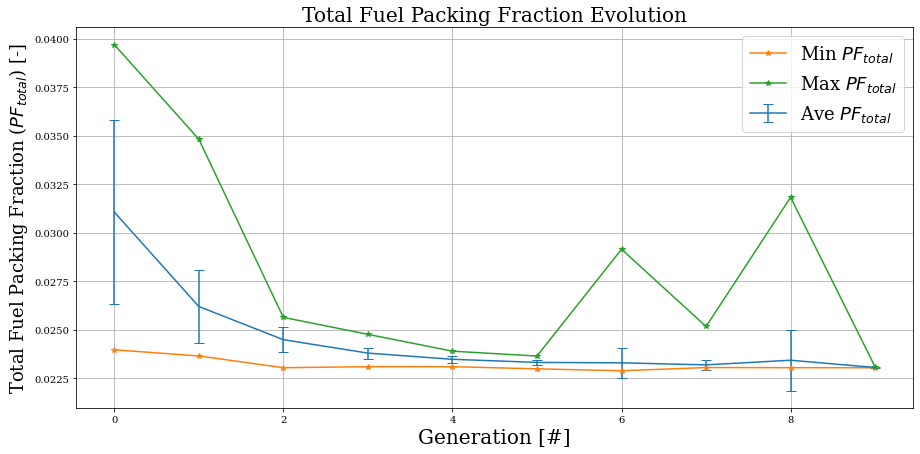
\includegraphics[width=\linewidth]{slab-obj-1-pf-evol.png}
        \caption{Minimum, average, and maximum $PF_{total}$ evolution.}
        \label{fig:slab-obj-1-pf-evol} 
    \end{subfigure}
    \begin{subfigure}{0.9\textwidth}
        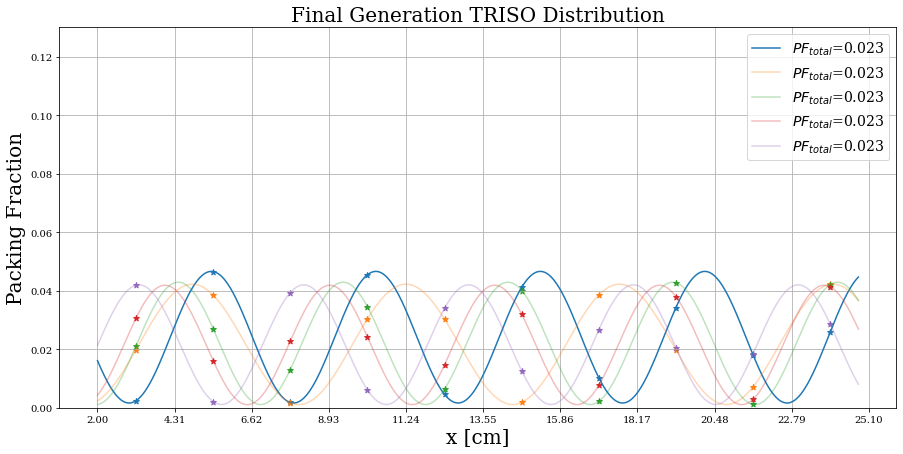
\includegraphics[width=\linewidth]{slab-obj-1-pf-final.png}
        \caption{TRISO packing fraction distribution for the 5 reactor models with the 
        smallest $PF_{total}$ in the final generation.}
        \label{fig:slab-obj-1-pf-final} 
    \end{subfigure}
    \begin{subfigure}{0.9\textwidth}
        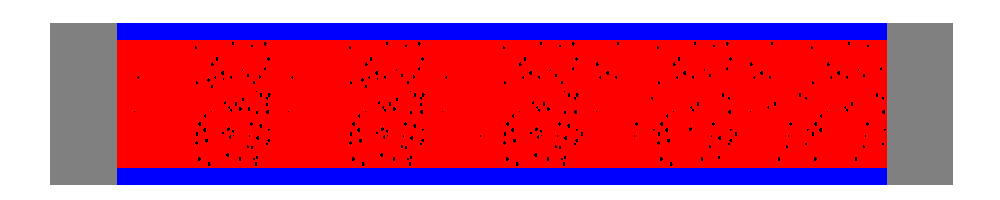
\includegraphics[width=\linewidth]{slab-obj-1-pf-most-minimized.png}
        \caption{\gls{AHTR} plank model with most-minimized $PF_{total}$ 
        (corresponds to the blue bolded distribution in the above plot).}
        \label{fig:slab-obj-1-pf-most-minimized} 
    \end{subfigure}
    \caption{Simulation p-1a -- ROLLO single-objective optimization to minimize total 
    fuel packing fraction ($PF_{total}$). 
    Input parameters varied: total fuel packing fraction 
    ($PF_{total}$), \gls{TRISO} packing fraction distribution ($\rho_{TRISO}(\vec{r})$).}
    \label{fig:slab-obj-1-pf}
\end{figure}

Figure \ref{fig:slab-obj-1-pf-evol} shows that the minimum and average $PF_{total}$ 
converged very quickly, as expected in this single-objective optimization 
problem.
By the final generation, the average, minimum, and maximum $PF_{total}$
values converged to approximately 0.023. 
In Figure \ref{fig:slab-obj-1-pf-final}, the \gls{TRISO} packing fraction
sine distributions are not exactly the same, but follow a similar pattern of 
alternating between a higher packing fraction, and a lower packing fraction 
in the neighboring fuel cell. 

Section \ref{sec:plank-discussion-pf} provides discussion about the motivating factors 
for the minimize $PF_{total}$ objective. 

\subsubsection{Simulation p-1d: Variation of $PF_{total}$ and Coolant channel shape}
Table \ref{tab:simulationp1d} shows simulation p-1d's optimization problem parameters. 
\begin{table}[htbp!]
    \centering
    \onehalfspacing
    \caption{Simulation p-1d Optimization Problem Parameters}
	\label{tab:simulationp1d}
    \footnotesize
    \begin{tabular}{l|p{5cm}}
    \hline 
    \multicolumn{2}{c}{\textbf{Single Objective: Simulation p-1d}} \\
    \hline 
    \textbf{Objectives} & Minimize $PF_{total}$\\
    \hline 
    \textbf{Input parameter variations} & $0.02<PF_{total}<0.05$ \\
    & $0.05<r_{top}<0.35$ \\
    & $0.05<r_{bot}<0.35$ \\
    \hline
    \textbf{Constraints} & $k_{eff} \geq 1.35$\\ 
    \hline 
    \textbf{Genetic algorithm parameters} & Population size: 64 \\
    & Generations: 3 \\
    \hline
    \end{tabular}
\end{table}

Figure \ref{fig:slab-obj-1-pf-evol-coolant} shows the $PF_{total}$ evolution 
and Figure \ref{fig:slab-obj-1-pf-final-coolant} shows a plot of total radius 
($r_{top} + r_{bot}$) against $PF_{total}$. 
\begin{figure}[htbp!]
    \centering
    \begin{subfigure}{\textwidth}
        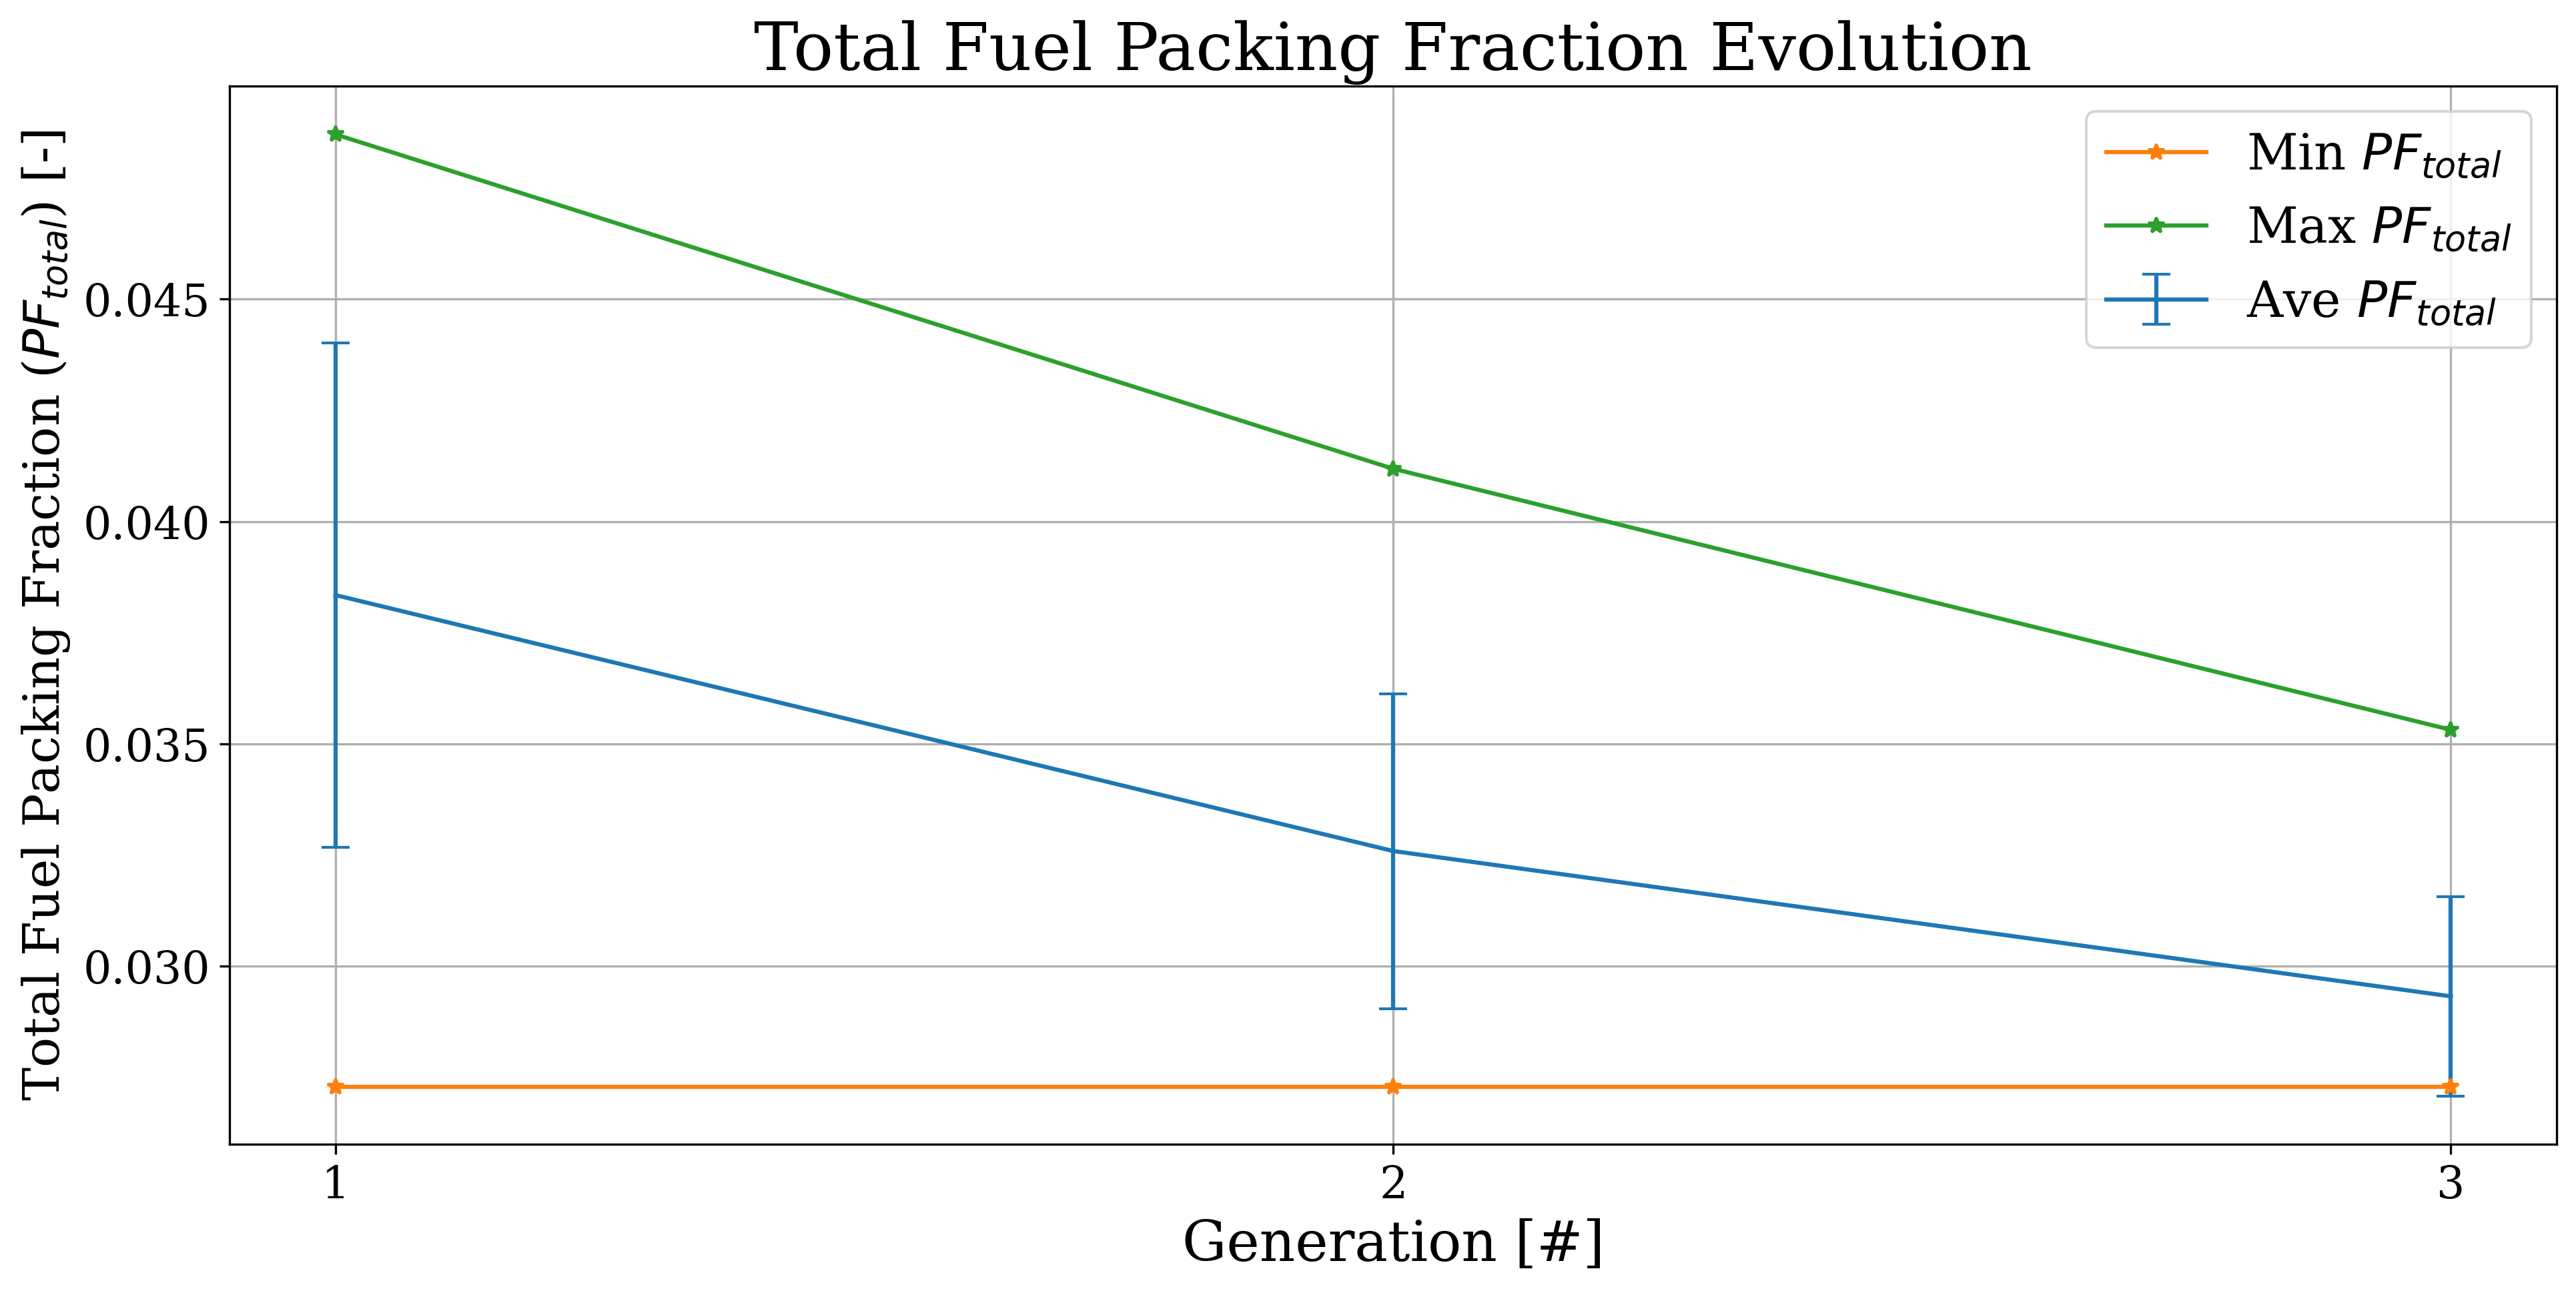
\includegraphics[width=\linewidth]{slab-obj-1-pf-evol-coolant.png}
        \caption{Minimum, average, and maximum total $PF_{total}$ evolution.}
        \label{fig:slab-obj-1-pf-evol-coolant} 
    \end{subfigure}
    \begin{subfigure}{\textwidth}
        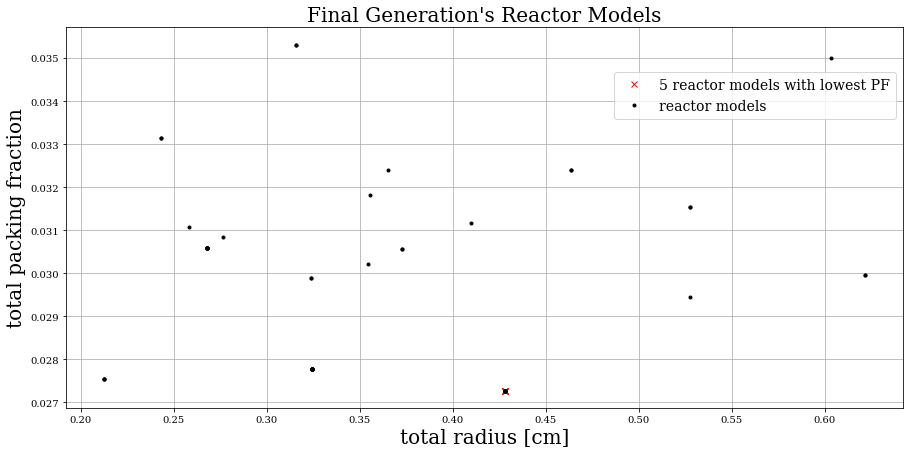
\includegraphics[width=\linewidth]{slab-obj-1-pf-final-coolant.png}
        \caption{Plot of total radius ($r_{top} + r_{bot}$) against $PF_{total}$. 
        Red crosses indicate the five reactor models with the 
        lowest $PF_{total}$.}
        \label{fig:slab-obj-1-pf-final-coolant} 
    \end{subfigure}
    \caption{Simulation p-1d -- ROLLO single-objective optimization to minimize 
    total fuel packing fraction. Input parameters varied: total fuel packing fraction 
    ($PF_{total}$), and coolant channel shape ($r_{top}, r_{bot}$).}
    \label{fig:slab-obj-1-pf-coolant}
\end{figure}
Figure \ref{fig:slab-obj-1-pf-final-coolant} demonstrates that there is no correlation 
between $PF_{total}$ and total radius. 

\subsection{Objective: Minimize Maximum Plank Temperature ($T_{max}$)}
\label{sec:plank-1-obj-temp}
This section reports results from the minimize maximum plank temperature 
($T_{max}$) single-objective optimization simulations: p-1b and p-1e. 
Simulation p-1b varies \gls{TRISO} packing fraction distribution 
($\rho_{TRISO}(\vec{r})$), while simulation p-1e varies the coolant channel shape. 

\subsubsection{Simulation p-1b: Variation of $\rho_{TRISO}(\vec{r})$}
Table \ref{tab:simulationp1b} shows simulation p-1b's optimization problem parameters. 
\begin{table}[htbp!]
    \centering
    \onehalfspacing
    \caption{Simulation p-1b Optimization Problem Parameters}
	\label{tab:simulationp1b}
    \footnotesize
    \begin{tabular}{l|p{3cm}}
    \hline 
    \multicolumn{2}{c}{\textbf{Single Objective: Simulation p-1b}} \\
    \hline 
    \textbf{Objectives} & Minimize $T_{max}$ \\
    \hline 
    \textbf{Input parameter variations} & $0<a<2$ \\
    & $0<b<\frac{\pi}{2}$ \\
    & $0<c<2\pi$ \\
    \hline
    \textbf{Constraints} & $k_{eff} \geq 1.0$\\ 
    & $PF_{total}$ = 0.0979\\
    \hline 
    \textbf{Genetic algorithm parameters} & Population size: 60 \\
    & Generations: 10 \\
    \hline
    \end{tabular}
\end{table}

Figure \ref{fig:slab-obj-1-temp-evol} shows the plank's $T_{max}$ evolution, Figure 
\ref{fig:slab-obj-1-temp-final} shows the five \gls{TRISO} packing fraction
distributions ($\rho_{TRISO}(\vec{r})$) in the final generation with the 
most-minimized $T_{max}$, and 
Figure \ref{fig:slab-obj-1-temp-most-minimized} illustrates the \gls{AHTR} plank model 
with most-minimized $T_{max}$. 
\begin{figure}[htbp!]
    \centering
    \begin{subfigure}{0.9\textwidth}
        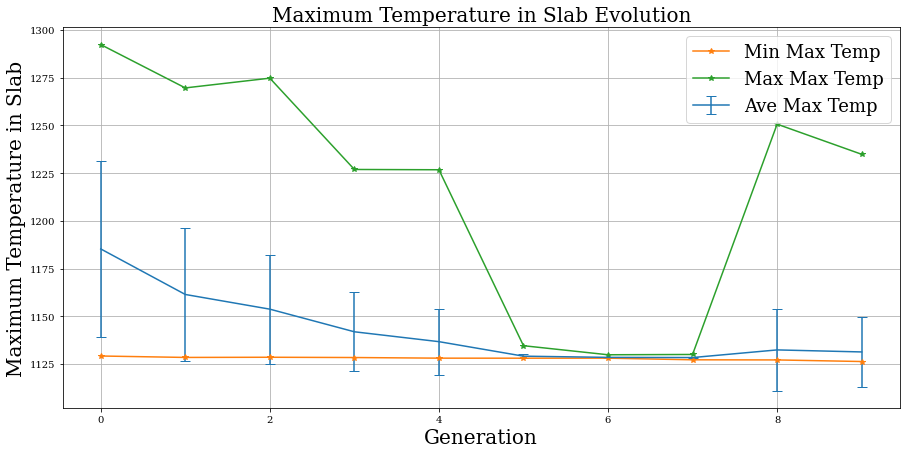
\includegraphics[width=\linewidth]{slab-obj-1-temp-evol.png}
        \caption{Minimum, average, and maximum evolution of AHTR plank's $T_{max}$.}
        \label{fig:slab-obj-1-temp-evol} 
    \end{subfigure}
    \begin{subfigure}{0.9\textwidth}
        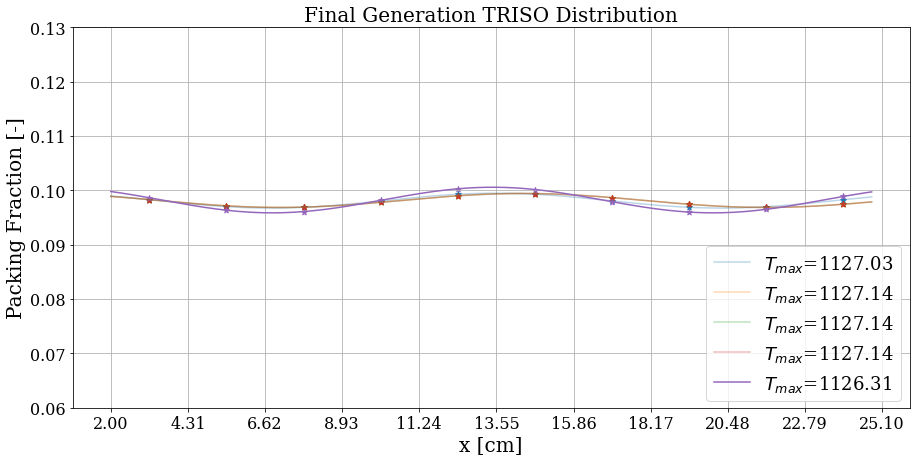
\includegraphics[width=\linewidth]{slab-obj-1-temp-final.png}
        \caption{TRISO distribution for the 5 reactor models with the 
        lowest AHTR plank $T_{max}$ at the final generation.}
        \label{fig:slab-obj-1-temp-final} 
    \end{subfigure}
    \begin{subfigure}{0.9\textwidth}
        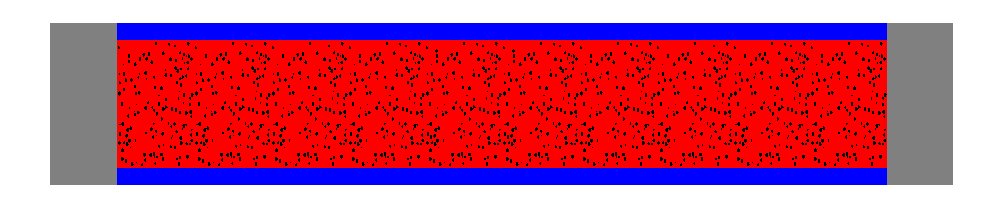
\includegraphics[width=\linewidth]{slab-obj-1-temp-most-minimized.png}
        \caption{\gls{AHTR} plank model with most-minimized $T_{max}$
        (corresponds to the purple bolded distribution in the above plot).}
        \label{fig:slab-obj-1-temp-most-minimized} 
    \end{subfigure}
    \caption{Simulation p-1b -- ROLLO single-objective optimization to minimize 
    maximum plank temperature ($T_{max}$). Input parameters varied: TRISO 
    packing fraction distribution ($\rho_{TRISO}(\vec{r})$). $PF_{total}$ = 0.0979.}
    \label{fig:slab-obj-1-temp}
\end{figure}

Figure \ref{fig:slab-obj-1-temp-evol} shows that the minimum and average plank's 
$T_{max}$ converged to approximately 1125 K. 
In Figure \ref{fig:slab-obj-1-temp-final}, a mostly flat TRISO
distribution minimizes $T_{max}$ in the plank, the TRISO distribution 
has two small dips at the one-third and two-third points in the plank 
(6.62cm and 20.48cm). 

Section \ref{sec:plank-discussion-temp} provides discussion about the motivating factors 
for the minimize $T_{max}$ objective. 

\subsubsection{Simulation p-1e: Variation of Coolant Channel Shape}
Table \ref{tab:simulationp1e} shows simulation p-1e's optimization problem parameters. 
\begin{table}[htbp!]
    \centering
    \onehalfspacing
    \caption{Simulation p-1e Optimization Problem Parameters}
	\label{tab:simulationp1e}
    \footnotesize
    \begin{tabular}{l|p{3cm}}
    \hline 
    \multicolumn{2}{c}{\textbf{Single Objective: Simulation p-1e}} \\
    \hline 
    \textbf{Objectives} & Minimize $T_{max}$ \\
    \hline 
    \textbf{Input parameter variations} & $0.05<r_{top}<0.35$ \\
    & $0.05<r_{bot}<0.35$ \\
    \hline
    \textbf{Constraints} & $k_{eff} \geq 1.35$\\ 
    & $PF_{total}$ = 0.0979\\
    \hline 
    \textbf{Genetic algorithm parameters} & Population size: 64 \\
    & Generations: 4 \\
    \hline
    \end{tabular}
\end{table}

Figure \ref{fig:slab-obj-1-temp-evol-coolant} shows the plank's $T_{max}$ evolution, 
Figure \ref{fig:slab-obj-1-temp-final-coolant} shows a plot of total radius 
($r_{top} + r_{bot}$) against $T_{max}$, and Figure 
\ref{fig:slab-obj-1-temp-most-minimized-coolant} illustrates the \gls{AHTR} plank model 
with most-minimized $T_{max}$. 
\begin{figure}[htbp!]
    \centering
    \begin{subfigure}{\textwidth}
        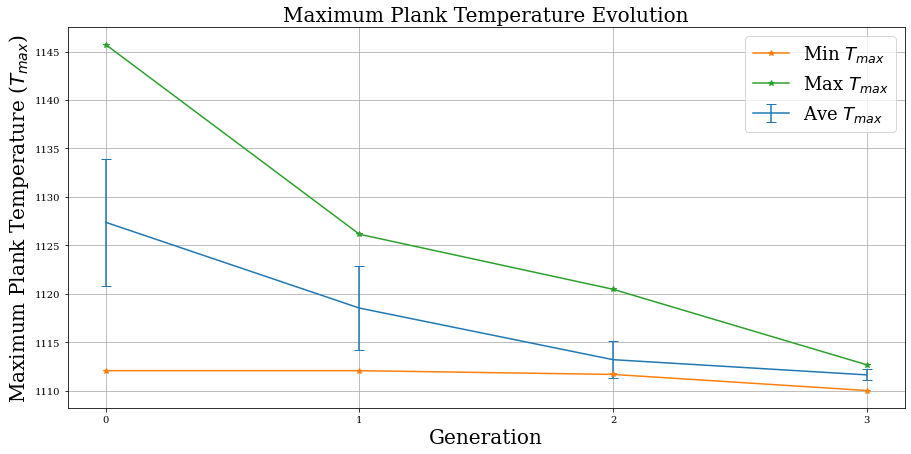
\includegraphics[width=\linewidth]{slab-obj-1-temp-evol-coolant.png}
        \caption{Minimum, average, and maximum evolution of AHTR plank's $T_{max}$.}
        \label{fig:slab-obj-1-temp-evol-coolant} 
    \end{subfigure}
    \begin{subfigure}{\textwidth}
        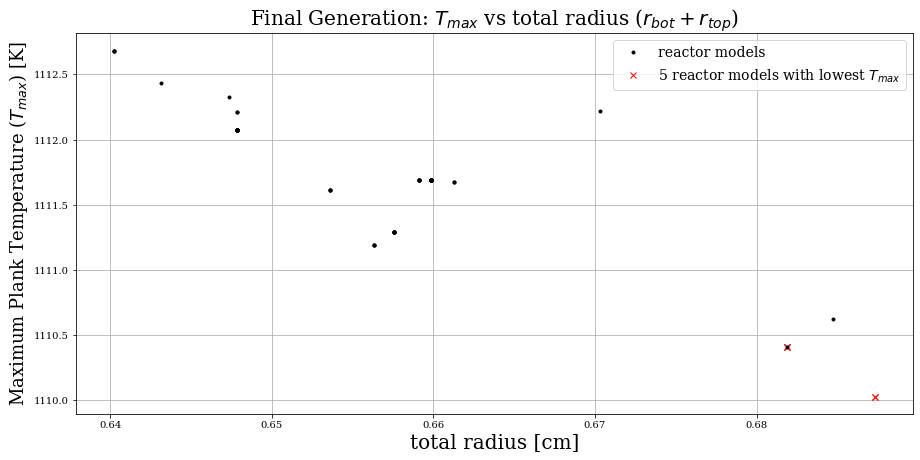
\includegraphics[width=\linewidth]{slab-obj-1-temp-final-coolant.png}
        \caption{Plot of total radius ($r_{top} + r_{bot}$) against plank's 
        $T_{max}$. Red crosses indicate the five reactor models with the 
        lowest $T_{max}$.}
        \label{fig:slab-obj-1-temp-final-coolant} 
    \end{subfigure}
    \begin{subfigure}{\textwidth}
        
\includegraphics[width=\linewidth]{slab-obj-1-temp-most-minimized-coolant.png}
        \caption{\gls{AHTR} plank model with most-minimized $T_{max}$. 
        $r_{top} = 0.337$ and $r_{bot} = 0.344$.}
        \label{fig:slab-obj-1-temp-most-minimized-coolant} 
    \end{subfigure}
    \caption{Simulation p-1e -- ROLLO single-objective optimization to minimize 
    maximum plank temperature ($T_{max}$). Input parameters varied: coolant channel shape 
    ($r_{top}, r_{bot}$). $PF_{total}$ = 0.0979.}
    \label{fig:slab-obj-1-temp-coolant}
\end{figure}

Figure \ref{fig:slab-obj-1-temp-final-coolant} demonstrates that there is a negative 
linear correlation between the plank's $T_{max}$ and total radius. 

Section \ref{sec:plank-discussion-temp} provides discussion about the motivating factors 
for the minimize $T_{max}$ objective. 

\subsection{Objective: Minimize Fuel-Normalized Power Peaking Factor ($PPF_{fuel}$)}
\label{sec:plank-1-obj-ppf}
This section reports results from the minimize fuel-normalized power peaking factor 
($PPF_{fuel}$) single-objective optimization simulations: p-1c and p-1f. 
Simulation p-1c varies \gls{TRISO} packing fraction distribution 
($\rho_{TRISO}(\vec{r})$), while simulation p-1f varies the coolant channel shape. 

\subsubsection{Simulation p-1c: Variation of $\rho_{TRISO}(\vec{r})$}
Table \ref{tab:simulationp1c} shows simulation p-1c's optimization problem parameters. 
\begin{table}[htbp!]
    \centering
    \onehalfspacing
    \caption{Simulation p-1c Optimization Problem Parameters}
	\label{tab:simulationp1c}
    \footnotesize
    \begin{tabular}{l|p{3cm}}
    \hline 
    \multicolumn{2}{c}{\textbf{Single Objective: Simulation p-1c}} \\
    \hline 
    \textbf{Objectives} & Minimize $PPF_{fuel}$ \\
    \hline 
    \textbf{Input parameter variations} & $0<a<2$ \\
    & $0<b<\frac{\pi}{2}$ \\
    & $0<c<2\pi$ \\
    \hline
    \textbf{Constraints} & $k_{eff} \geq 1.0$\\ 
    & $PF_{total}$ = 0.0979\\
    \hline 
    \textbf{Genetic algorithm parameters} & Population size: 60 \\
    & Generations: 10 \\
    \hline
    \end{tabular}
\end{table}

Figure \ref{fig:slab-obj-1-ppf-evol} shows the plank's $PPF_{fuel}$ evolution, 
Figure \ref{fig:slab-obj-1-ppf-final} shows the five \gls{TRISO} 
packing fraction distributions ($\rho_{TRISO}(\vec{r})$) in the final generation 
with the most-minimized $PPF_{fuel}$, and Figure 
\ref{fig:slab-obj-1-ppf-most-minimized} illustrates the \gls{AHTR} plank model with 
most-minimized $PPF_{fuel}$. 
\begin{figure}[htbp!]
    \centering
    \begin{subfigure}{0.9\textwidth}
        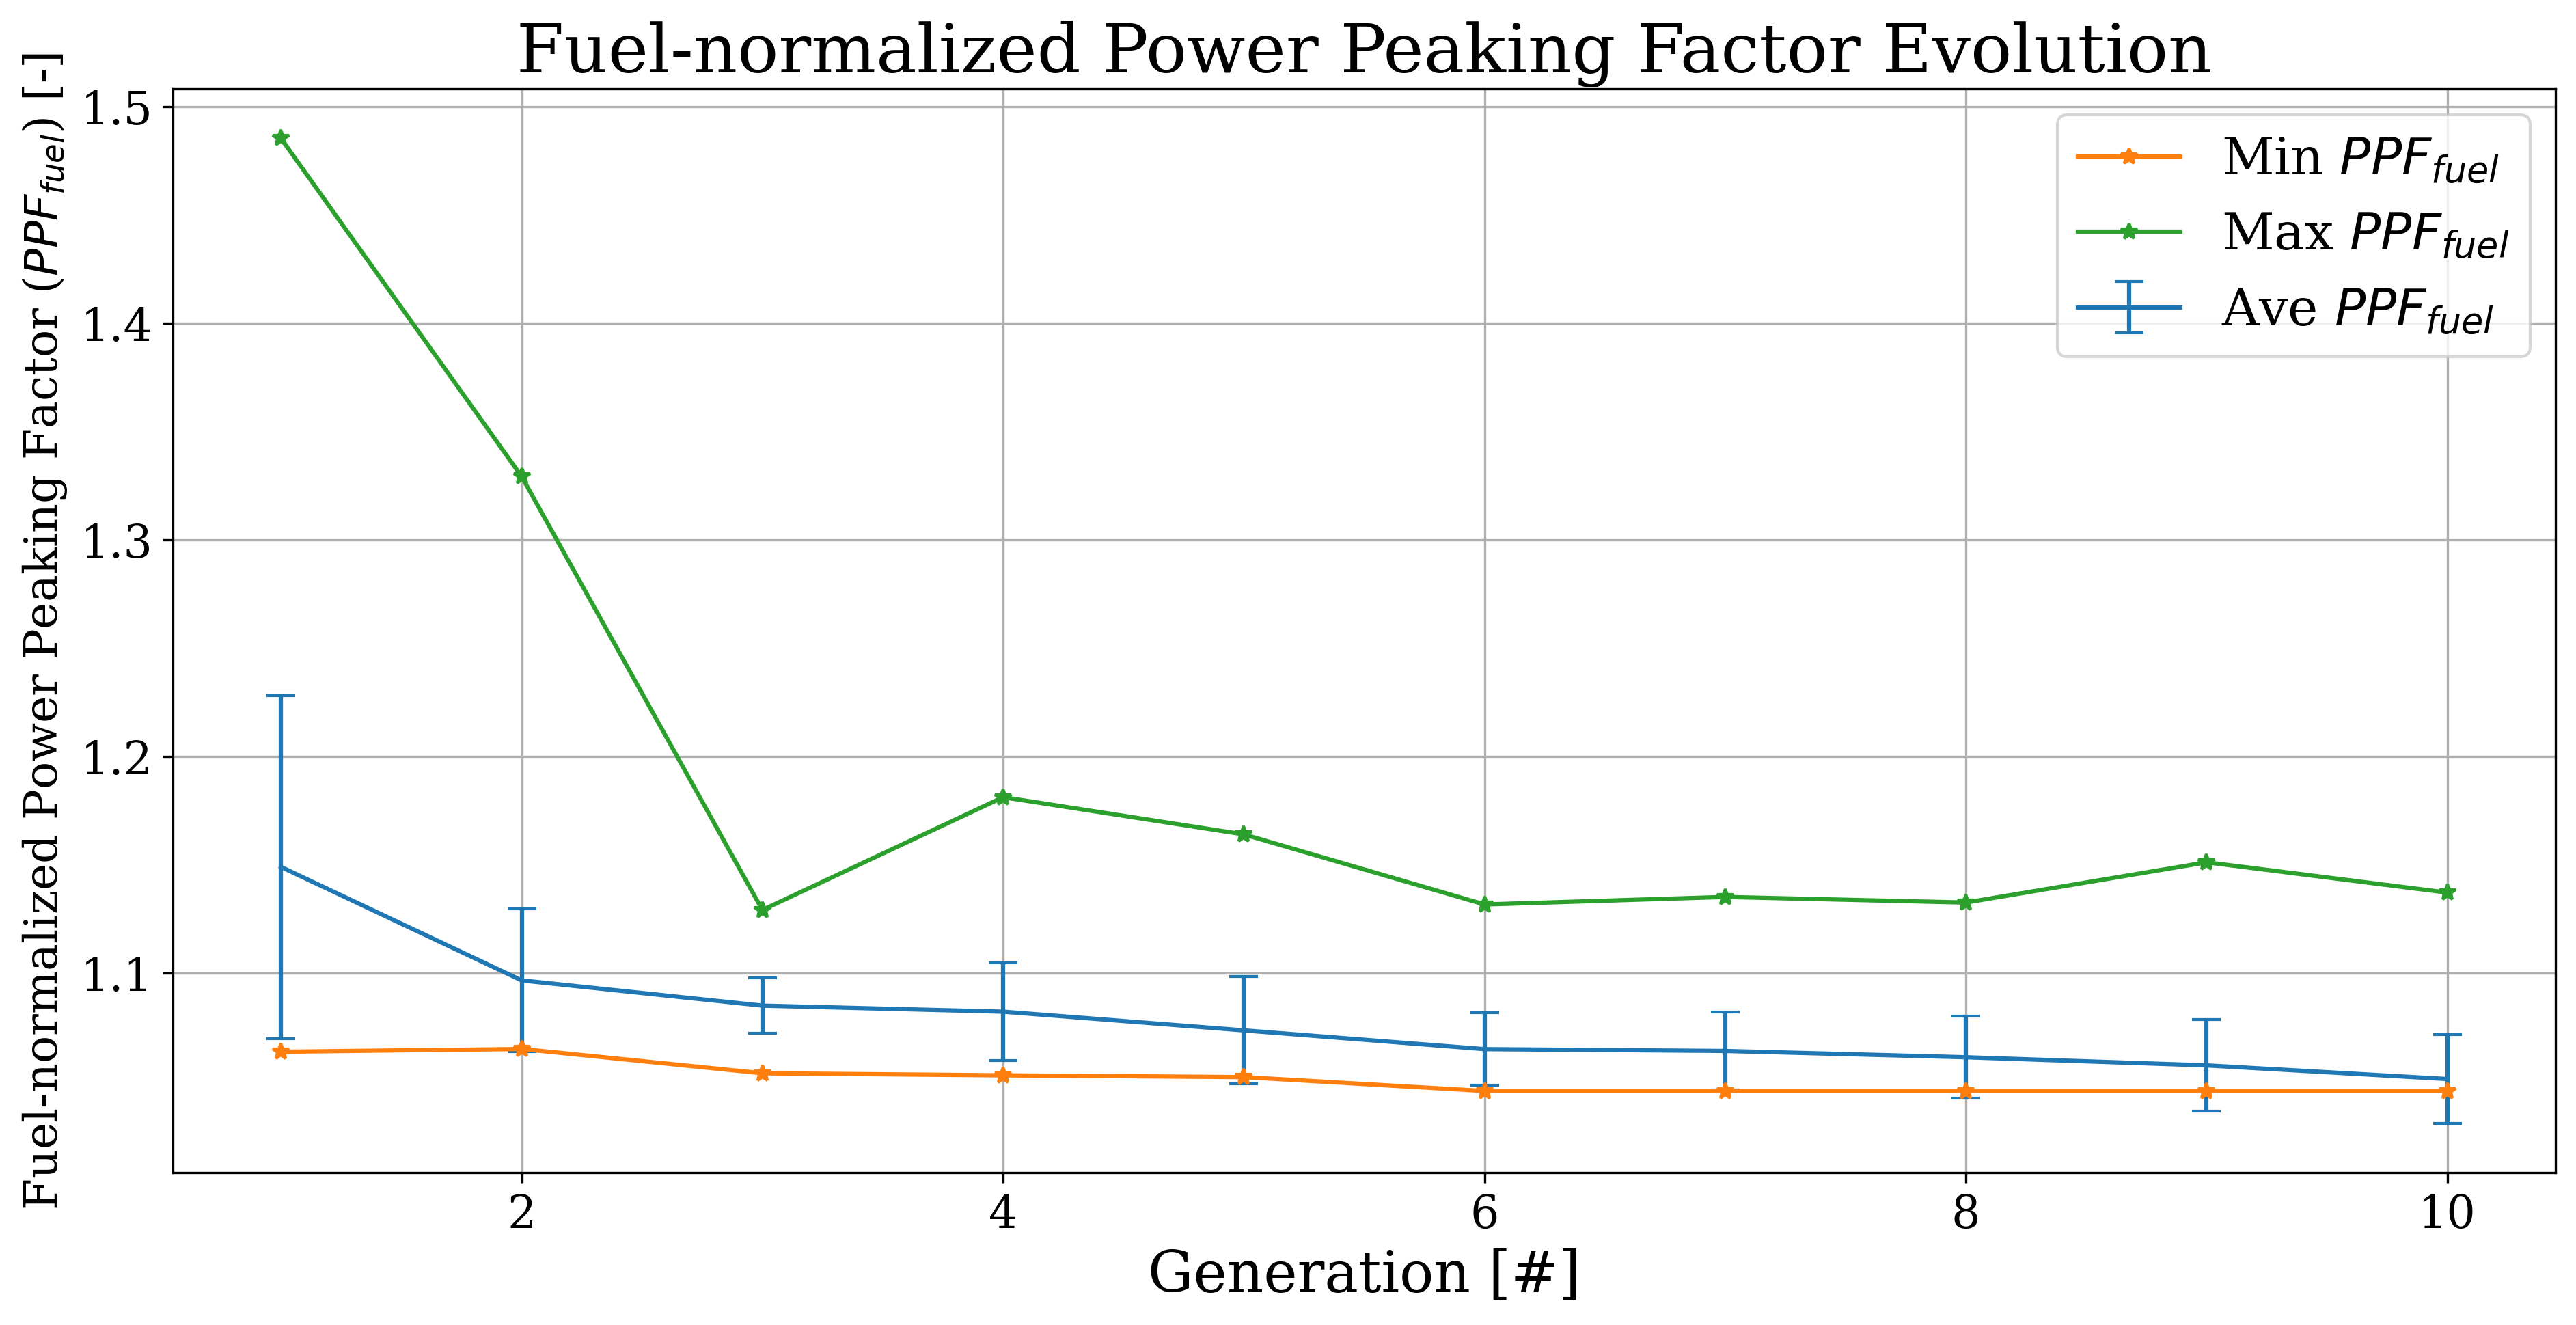
\includegraphics[width=\linewidth]{slab-obj-1-ppf-evol.png}
        \caption{Minimum, average, and maximum evolution of $PPF_{fuel}$ in the 
        AHTR plank.}
        \label{fig:slab-obj-1-ppf-evol} 
    \end{subfigure}
    \begin{subfigure}{0.9\textwidth}
        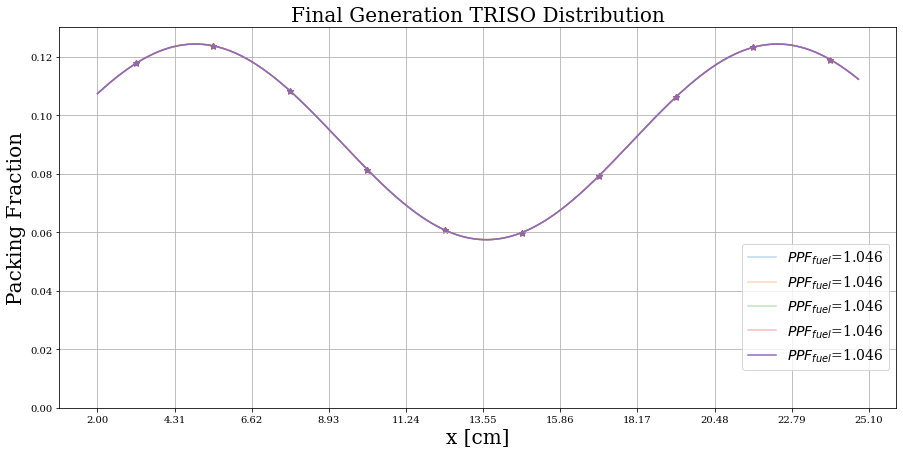
\includegraphics[width=\linewidth]{slab-obj-1-ppf-final.png}
        \caption{TRISO distribution for the 5 reactor models with the 
        lowest $PPF_{fuel}$ in AHTR plank at the final generation.}
        \label{fig:slab-obj-1-ppf-final} 
    \end{subfigure}
    \begin{subfigure}{0.9\textwidth}
        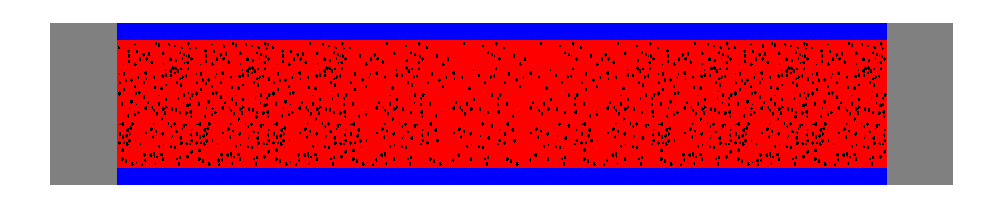
\includegraphics[width=\linewidth]{slab-obj-1-ppf-most-minimized.png}
        \caption{\gls{AHTR} plank model with most-minimized $PPF_{fuel}$
        (corresponds to the purple bolded distribution in the above plot).}
        \label{fig:slab-obj-1-ppf-most-minimized} 
    \end{subfigure}
    \caption{Simulation p-1c -- ROLLO single-objective optimization to minimize 
    AHTR plank's fuel-normalized power peaking factor ($PPF_{fuel}$). 
    Input parameters varied: TRISO distribution ($\rho_{TRISO}(\vec{r})$).
    $PF_{total}$ = 0.0979.}
    \label{fig:slab-obj-1-ppf}
\end{figure}

In Figure \ref{fig:slab-obj-1-ppf-final}, the TRISO distribution that best minimizes 
$PPF_{fuel}$ peaks near the edges of the fuel region of the plank, and has a minimum 
point in center of the plank.

Section \ref{sec:plank-discussion-ppf} provides discussion about the motivating factors 
for the minimize $PPF_{fuel}$ objective. 

\subsubsection{Simulation p-1f: Variation of Coolant Channel Shape}
Table \ref{tab:simulationp1f} shows simulation p-1f's optimization problem parameters. 
\begin{table}[htbp!]
    \centering
    \onehalfspacing
    \caption{Simulation p-1f Optimization Problem Parameters}
	\label{tab:simulationp1f}
    \footnotesize
    \begin{tabular}{l|p{3cm}}
    \hline 
    \multicolumn{2}{c}{\textbf{Single Objective: Simulation p-1f}} \\
    \hline 
    \textbf{Objectives} & Minimize $PPF_{fuel}$ \\
    \hline 
    \textbf{Input parameter variations} & $0.05<r_{top}<0.35$ \\
    & $0.05<r_{bot}<0.35$ \\
    \hline
    \textbf{Constraints} & $k_{eff} \geq 1.35$\\ 
    & $PF_{total}$ = 0.0979\\
    \hline 
    \textbf{Genetic algorithm parameters} & Population size: 64 \\
    & Generations: 5 \\
    \hline
    \end{tabular}
\end{table}

Figure \ref{fig:slab-obj-1-ppf-evol-coolant} shows the plank's $PPF_{fuel}$ evolution 
and Figure \ref{fig:slab-obj-1-ppf-final-coolant} shows a plot of total 
radius ($r_{top} + r_{bot}$) against $PPF_{fuel}$. 
\begin{figure}[htbp!]
    \centering
    \begin{subfigure}{\textwidth}
        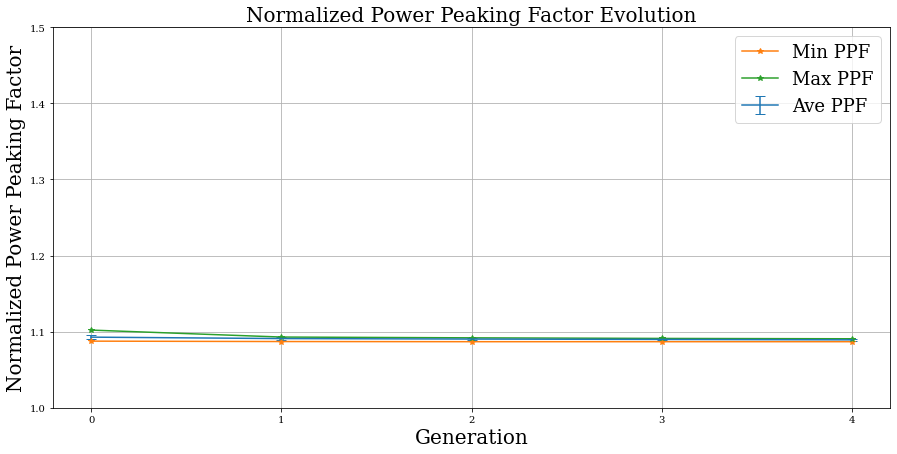
\includegraphics[width=\linewidth]{slab-obj-1-ppf-evol-coolant.png}
        \caption{Minimum, average, and maximum evolution of $PPF_{fuel}$ in the 
        AHTR plank.}
        \label{fig:slab-obj-1-ppf-evol-coolant} 
    \end{subfigure}
    \begin{subfigure}{\textwidth}
        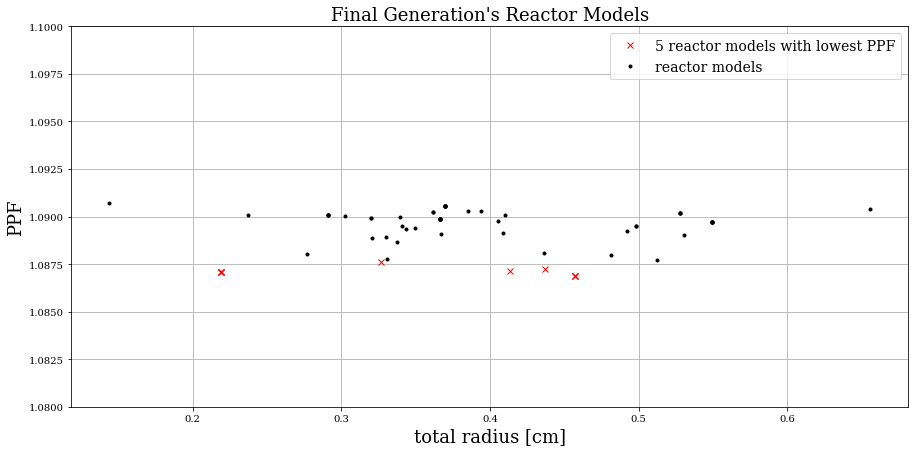
\includegraphics[width=\linewidth]{slab-obj-1-ppf-final-coolant.png}
        \caption{Plot of total radius ($r_{top} + r_{bot}$) against $PPF_{fuel}$. 
        Red crosses indicate the five reactor models with the lowest $PPF_{fuel}$.}
        \label{fig:slab-obj-1-ppf-final-coolant} 
    \end{subfigure}
    \caption{Simulation p-1f -- ROLLO single-objective optimization to minimize 
    fuel-normalized power peaking factor ($PPF_{fuel}$) in the slab. 
    Input parameters varied: coolant channel shape ($r_{top}, r_{bot}$). 
    $PF_{total}$ = 0.0979.}
    \label{fig:slab-obj-1-ppf-coolant}
\end{figure}

% description? 
Section \ref{sec:plank-discussion-ppf} provides discussion about the motivating factors 
for the minimize $PPF_{fuel}$ objective. 


\pagebreak
\section{AHTR Plank: Two-Objective Optimization Results}
In this section, I report the \gls{AHTR} plank's \gls{ROLLO} two-objective 
optimization results. 
The previous section's one-objective optimization results inform the multi-objective 
optimization simulations in this section and Section \ref{sec:plank-three-obj}.
Since the variations in coolant channel shape does not impact two out of three objectives: 
minimize total packing fraction and minimize fuel-normalized power peaking factor 
objectives, I do not conduct two-objective optimization for coolant channel shape 
variations.  
Table \ref{tab:slab-obj-breakdown} summarized the two-objective simulations in this 
section: p-2a, p-2b, and p-2c.

As previously described in Section \ref{sec:opt}, multi-objective optimization returns 
multiple optimal solutions that meet each objective to varying degrees; this set of 
solutions is the Pareto front \cite{deb_multi-objective_2001}. 
For each solution in the Pareto front, none of the objective functions can be 
improved without degrading another objective.
An ideal optimization method for a multi-objective problem like reactor design 
should find widely spread solutions in the obtained Pareto front 
\cite{deb_multi-objective_2001}. 
Thus, I report on the optimal reactor models on the Pareto front for the multi-objective 
optimization problems in this section and Section \ref{sec:plank-three-obj}. 

To ensure that the multi-objective optimization problems are converged, I report the 
hypervolume values for each generation. 
As previously described in Section \ref{sec:binhandkorn}, the hypervolume indicator 
quantifies the Pareto front's goodness (bigger = better).
I use a different reference point for each optimization problem. 
If a multi-objective optimization problem's hypervolume converges earlier than the 
5 generations I intended to run (determined in Section 
\ref{sec:multi-obj-hyperparameters}), I stop running the simulation at that generation. 
However, if the multi-objective optimization problem's hypervolume does not converge by 
generation 5, I run the problem for a few more generations till satisfactory convergence.

\subsection{p-2a: Minimize $PF_{total}$ and $T_{max}$}
\label{sec:p-2a}
This section reports results from the two-objective optimization simulation p-2a, the 
objectives minimized are total fuel packing fraction ($PF_{total}$) and maximum plank
temperature ($T_{max}$).  
Table \ref{tab:simulationp2a} shows simulation p-2a's optimization problem parameters.
\begin{table}[htbp!]
    \centering
    \onehalfspacing
    \caption{Simulation p-2a Optimization Problem Parameters.}
	\label{tab:simulationp2a}
    \footnotesize
    \begin{tabular}{l|p{4cm}}
    \hline 
    \multicolumn{2}{c}{\textbf{Two Objectives: Simulation p-2a}} \\
    \hline 
    \textbf{Objectives} & Minimize $PF_{total}$ \\
    & Minimize $T_{max}$ \\
    \hline 
    \textbf{Input parameter variations} & $0.02<PF_{total}<0.04$ \\
    & $0<a<2$ \\
    & $0<b<\frac{\pi}{2}$ \\
    & $0<c<2\pi$ \\
    \hline
    \textbf{Constraints} & $k_{eff} \geq 1.35$\\ 
    \hline 
    \textbf{Genetic algorithm parameters} & Population size: 128 \\
    & Generations: 2 \\
    \hline
    \end{tabular}
\end{table}

Table \ref{tab:p2a-hypervolume} shows the hypervolume value at each generation, 
confirming that simulation p-2a converges by generation 2. 
\begin{table}[htbp!]
    \centering
    \onehalfspacing
    \caption{Simulation p-2a hypervolume values at each generation.}
	\label{tab:p2a-hypervolume}
    \footnotesize
    \begin{tabular}{ll}
    \hline 
    \multicolumn{2}{c}{\textbf{Two Objectives: Simulation p-2a}} \\
    \multicolumn{2}{c}{Reference point: (0.1, 1350)} \\
    \hline 
    \textbf{Generation} & \textbf{Hypervolume value} \\
    \hline
    1 & 17.659 \\
    2 & 17.659 \\
    \hline
    \end{tabular}
\end{table}

Figure \ref{fig:slab-obj-2-pftemp-pareto} shows a plot of the final generation's reactor 
models' $PF_{total}$ against $T_{max}$, crosses mark the reactor models that 
fall on the Pareto front.
Figure \ref{fig:slab-obj-2-pftemp-pareto-distr} shows the six TRISO distributions in 
the final generation that fall on the Pareto front.
Figures \ref{fig:slab-obj-2-pftemp-min-pf} and \ref{fig:slab-obj-2-pftemp-min-temp} 
illustrate the \gls{AHTR} plank models with most-minimized $PF_{total}$ and 
$T_{max}$, respectively.  
\begin{figure}[htbp!]
    \centering
    \begin{subfigure}{\textwidth}
        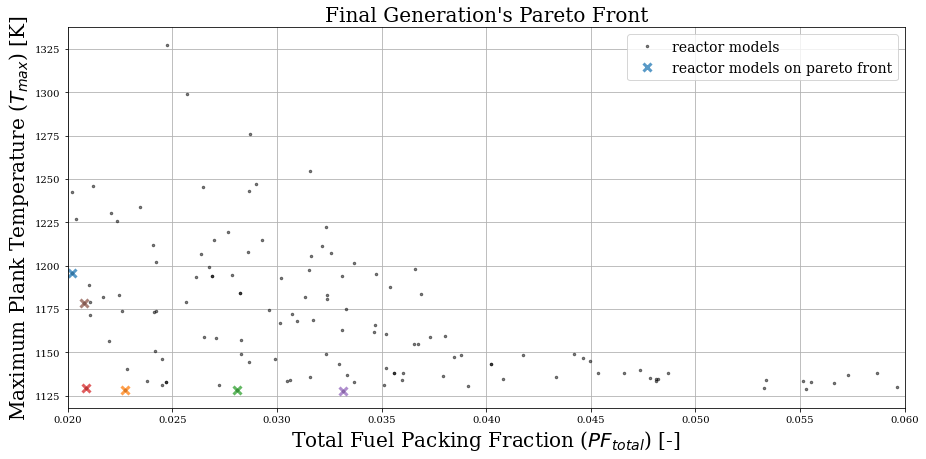
\includegraphics[width=\linewidth]{slab-obj-2-pftemp-pareto.png}
        \caption{Plot of final generation's reactor models' $PF_{total}$ against 
        $T_{max}$. Crosses indicate the reactor models on the Pareto front. 
        Cross colors correspond to TRISO distributions in the plot below.}
        \label{fig:slab-obj-2-pftemp-pareto} 
    \end{subfigure}
    \begin{subfigure}{\textwidth}
        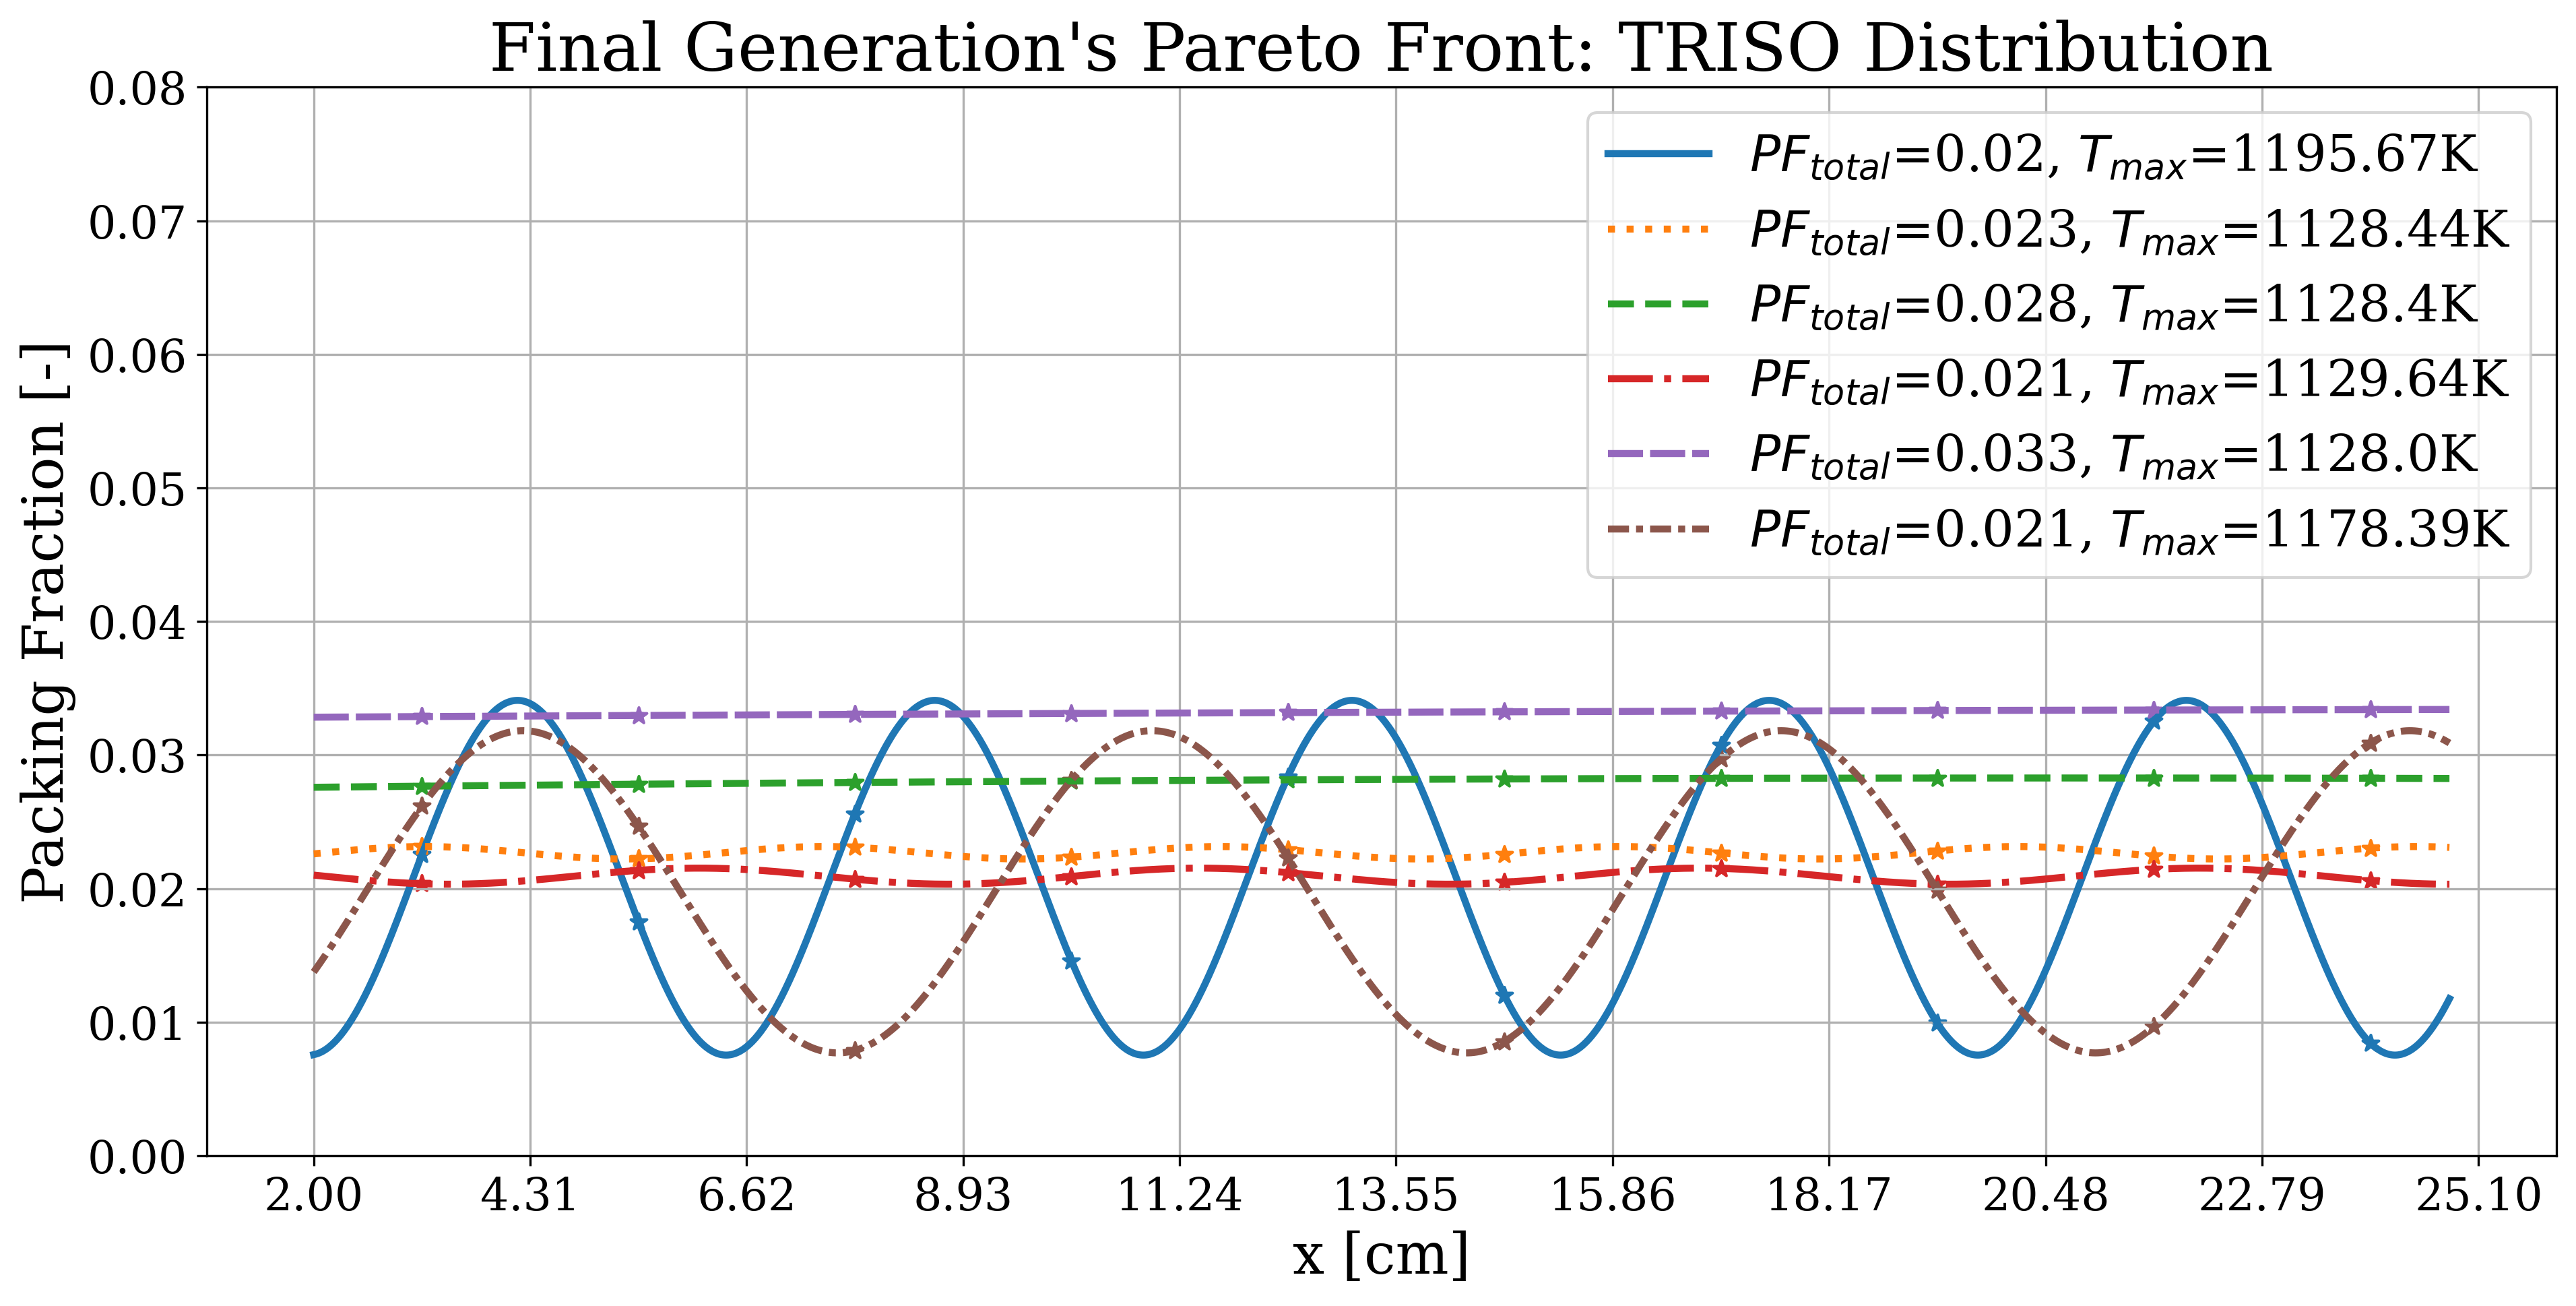
\includegraphics[width=\linewidth]{slab-obj-2-pftemp-pareto-distr.png}
        \caption{TRISO packing fraction distribution for the 6 reactor models on the 
        Pareto front.}
        \label{fig:slab-obj-2-pftemp-pareto-distr} 
    \end{subfigure}
    \caption{Simulation p-2a -- ROLLO two-objective optimization to minimize total 
    fuel packing fraction ($PF_{total}$) and maximum plank temperature ($T_{max}$). 
    Input parameters varied: total fuel packing fraction ($PF_{total}$) and 
    \gls{TRISO} distribution ($\rho_{TRISO}(\vec{r})$).}
    \label{fig:slab-obj-2-pftemp}
\end{figure}
\begin{figure}[htbp!]
    \ContinuedFloat
    \begin{subfigure}{\textwidth}
        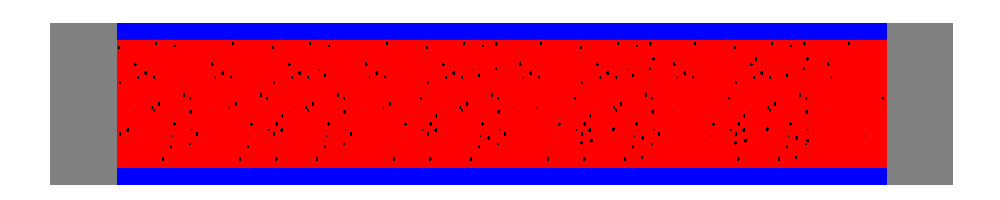
\includegraphics[width=\linewidth]{slab-obj-2-pftemp-min-pf.png}
        \caption{\gls{AHTR} plank model with most-minimized $PF_{total}$
        (corresponds to the blue bolded distribution in Figure 
        \ref{fig:slab-obj-2-pftemp-pareto-distr}).}
        \label{fig:slab-obj-2-pftemp-min-pf} 
    \end{subfigure}
    \begin{subfigure}{\textwidth}
        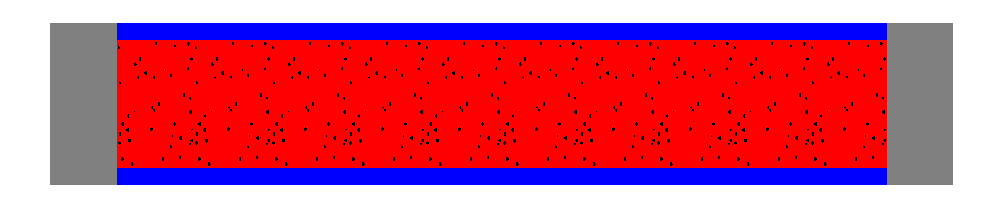
\includegraphics[width=\linewidth]{slab-obj-2-pftemp-min-temp.png}
        \caption{\gls{AHTR} plank model with most-minimized $T_{max}$
        (corresponds to the purple bolded distribution in Figure 
        \ref{fig:slab-obj-2-pftemp-pareto-distr}).}
        \label{fig:slab-obj-2-pftemp-min-temp} 
    \end{subfigure}
    \caption{(contd.) Simulation p-2a -- ROLLO two-objective optimization to minimize 
    total packing fraction ($PF_{total}$) and maximum plank temperature ($T_{max}$). 
    Input parameters varied: total fuel packing fraction ($PF_{total}$) and 
    \gls{TRISO} packing fraction distribution ($\rho_{TRISO}(\vec{r})$).}
\end{figure}

In Figure \ref{fig:slab-obj-2-pftemp-pareto-distr}, the TRISO distribution with the
most-minimized $PF_{total}$ and the highest $T_{max}$ (the blue distribution) has an 
oscillating TRISO distribution (also illustrated in Figure 
\ref{fig:slab-obj-2-pftemp-min-pf}).
This distribution is similar to simulation p-1a's most-minimized $PF_{total}$ TRISO 
distribution (Figure \ref{fig:slab-obj-1-pf-final}), but differs as it varies between 
0.005 and 0.035, instead of 0 and 0.4, due to influences from the minimize $T_{max}$ 
objective. 
In Figure \ref{fig:slab-obj-2-pftemp-pareto-distr}, the TRISO distribution with the 
most-minimized $T_{max}$ and highest $PF_{total}$ (the purple distribution)
has an almost constant packing fraction of $\sim0.032$ across the plank (also 
illustrated in Figure \ref{fig:slab-obj-2-pftemp-min-temp}). 
This distribution follows a similar flat shape as simulation p-1b's most-minimized 
$T_{max}$ TRISO distribution (Figure \ref{fig:slab-obj-1-temp-final}).

Thus, the \gls{TRISO} distributions on the Pareto front in Figure \ref{fig:slab-obj-2-pftemp} 
that minimizes both $PF_{total}$ and $T_{max}$ have varying degrees of flatness: 
the minimize $T_{max}$ objective influences the flatness and the minimize $PF_{total}$ 
objective influences the oscillating pattern. 

\subsection{p-2b: Minimize $PF_{total}$ and $PPF_{fuel}$}
\label{sec:p-2b}
This section reports results from the two-objective optimization simulation p-2b, the 
objectives minimized are total fuel packing fraction ($PF_{total}$) and fuel-normalized 
power peaking factor ($PPF_{fuel}$).  
Table \ref{tab:simulationp2b} shows simulation p-2b's optimization problem parameters. 
\begin{table}[htbp!]
    \centering
    \onehalfspacing
    \caption{Simulation p-2b Optimization Problem Parameters}
	\label{tab:simulationp2b}
    \footnotesize
    \begin{tabular}{l|p{3cm}}
    \hline 
    \multicolumn{2}{c}{\textbf{Two Objectives: Simulation p-2b}} \\
    \hline 
    \textbf{Objectives} & Minimize $PF_{total}$ \\
    & Minimize $PPF_{fuel}$ \\
    \hline 
    \textbf{Input parameter variations} & $0.02<PF_{total}<0.04$ \\
    & $0<a<2$ \\
    & $0<b<\frac{\pi}{2}$ \\
    & $0<c<2\pi$ \\
    \hline
    \textbf{Constraints} & $k_{eff} \geq 1.35$\\ 
    \hline 
    \textbf{Genetic algorithm parameters} & Population size: 128 \\
    & Generations: 3 \\
    \hline
    \end{tabular}
\end{table}

Table \ref{tab:p2b-hypervolume} shows the hypervolume value at each generation, 
confirming that simulation p-2b converges by generation 3. 
\begin{table}[htbp!]
    \centering
    \onehalfspacing
    \caption{Simulation p-2b hypervolume values at each generation.}
	\label{tab:p2b-hypervolume}
    \footnotesize
    \begin{tabular}{ll}
    \hline 
    \multicolumn{2}{c}{\textbf{Two Objectives: Simulation p-2b}} \\
    \multicolumn{2}{c}{Reference point: (0.1, 1.5)} \\
    \hline 
    \textbf{Generation} & \textbf{Hypervolume value} \\
    \hline
    1 & 0.03607 \\
    2 & 0.03619 \\
    3 & 0.03625 \\
    \hline
    \end{tabular}
\end{table}

Figure \ref{fig:slab-obj-2-pfppf-pareto} shows a plot of the final generation's reactor 
models' $PF_{total}$ against $PPF_{fuel}$, crosses mark the reactor models that fall on 
the Pareto front.
Figure \ref{fig:slab-obj-2-pfppf-pareto-distr} shows the four TRISO packing fraction 
distributions in the final generation that fall on the Pareto front. 
Figures \ref{fig:slab-obj-2-pfppf-min-pf} and \ref{fig:slab-obj-2-pfppf-min-ppf} 
illustrate the \gls{AHTR} plank models with most-minimized $PF_{total}$ and 
$PPF_{fuel}$, respectively. 
\begin{figure}[htbp!]
    \centering
    \begin{subfigure}{\textwidth}
        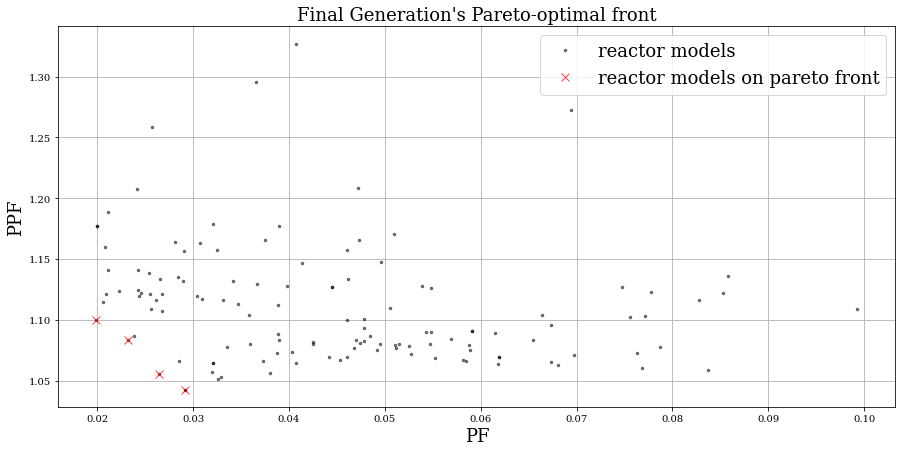
\includegraphics[width=\linewidth]{slab-obj-2-pfppf-pareto.png}
        \caption{Plot of final generation's reactor models' $PF_{total}$ against 
        $PPF_{fuel}$. 
        Crosses indicate the reactor models on the Pareto front. Cross colors correspond  
        to TRISO distributions in the plot below.}
        \label{fig:slab-obj-2-pfppf-pareto} 
    \end{subfigure}
    \begin{subfigure}{\textwidth}
        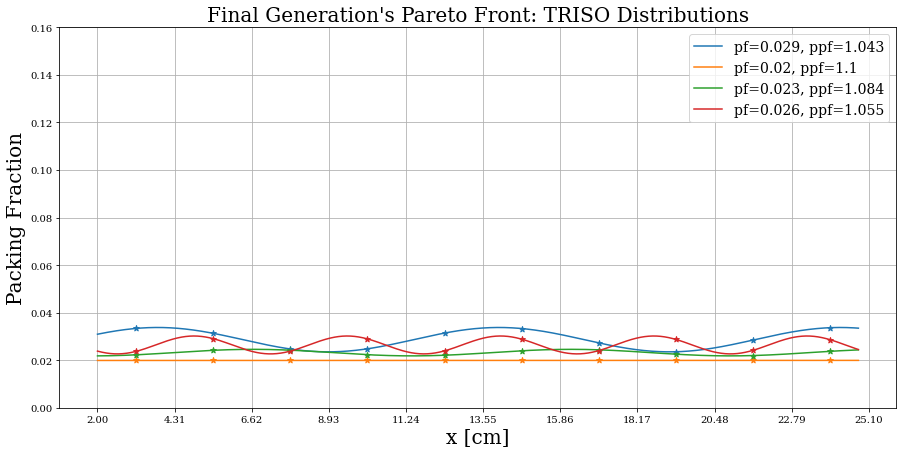
\includegraphics[width=\linewidth]{slab-obj-2-pfppf-pareto-distr.png}
        \caption{TRISO distribution for the 4 reactor models on the Pareto front.}
        \label{fig:slab-obj-2-pfppf-pareto-distr} 
    \end{subfigure}
    \caption{Simulation p-2b -- ROLLO two-objective optimization to minimize total fuel 
    packing fraction ($PF_{total}$) and normalized power peaking factor ($PPF_{fuel}$) 
    in the plank. 
    Input parameters varied: TRISO packing fraction distribution 
    ($\rho_{TRISO}(\vec{r})$).}
    \label{fig:slab-obj-2-pfppf}
\end{figure}
\begin{figure}[htbp!]
    \ContinuedFloat
    \begin{subfigure}{\textwidth}
        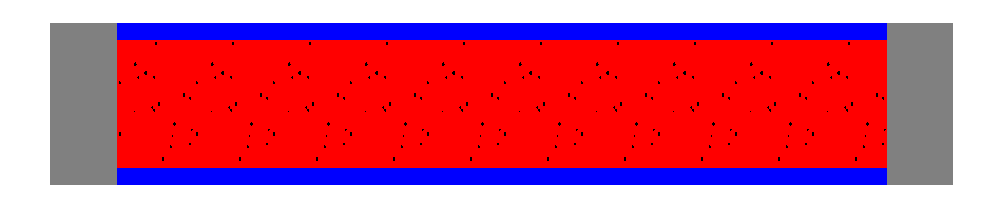
\includegraphics[width=\linewidth]{slab-obj-2-pfppf-min-pf.png}
        \caption{\gls{AHTR} plank model with most-minimized $PF_{total}$
        (corresponds to the orange bolded distribution in Figure 
        \ref{fig:slab-obj-2-pfppf-pareto-distr}).}
        \label{fig:slab-obj-2-pfppf-min-pf} 
    \end{subfigure}
    \begin{subfigure}{\textwidth}
        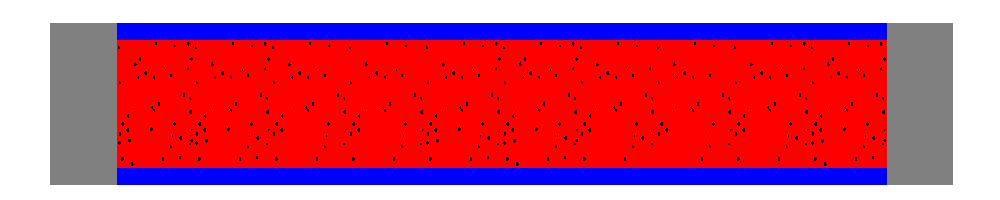
\includegraphics[width=\linewidth]{slab-obj-2-pfppf-min-ppf.png}
        \caption{\gls{AHTR} plank model with most-minimized $PPF_{fuel}$
        (corresponds to the blue bolded distribution in Figure 
        \ref{fig:slab-obj-2-pfppf-pareto-distr}).}
        \label{fig:slab-obj-2-pfppf-min-ppf} 
    \end{subfigure}
    \caption{(contd.) Simulation p-2b -- ROLLO two-objective optimization to minimize 
    total packing fraction ($PF_{total}$) and fuel-normalized power peaking factor 
    ($PPF_{fuel}$) in the plank. 
    Input parameters varied: TRISO packing fraction distribution ($\rho_{TRISO}(\vec{r})$).}
\end{figure}

All reactor models on Figure \ref{fig:slab-obj-2-pfppf}'s Pareto front have a relatively 
flat TRISO packing fraction distribution, varying between 0.02 and 0.04. 
In Figure \ref{fig:slab-obj-2-pfppf-pareto-distr}, the TRISO distribution with the 
most-minimized $PF_{total}$ and highest $PPF_{fuel}$
(the orange distribution) has a constant packing fraction of 0.02 across the plank
(also illustrated in Figure \ref{fig:slab-obj-2-pfppf-min-pf}). 
In Figure \ref{fig:slab-obj-2-pfppf-pareto-distr}, the TRISO distribution with the 
most-minimized $PPF_{fuel}$ and highest $PF_{total}$
(the blue distribution), has a packing fraction that peaks in the center of the plank
and both sides (also illustrated in Figure \ref{fig:slab-obj-2-pfppf-min-ppf}). 
This distribution differs from simulation p-1c's most-minimized $PPF_{fuel}$ TRISO 
distribution (Figure \ref{fig:slab-obj-1-ppf-final}) which has a large $\sim 0.06$ 
variation in TRISO distribution with a minimum point in the center of the plank . 
This difference is due to the different $PF_{total}$ values: simulation p-1c's total PF 
is 0.0979, while the total PF in the most-minimized $PPF_{fuel}$ model 
(blue distribution) is 0.029. 
In Section \ref{sec:p-2b-pf-ppf-study}, I perform a study of $PF_{total}$ 
and $PPF_{fuel}$ to gain a better understand their relationship. 

\subsubsection{Relationship Study: $PF_{total}$ and $PPF_{fuel}$}
\label{sec:p-2b-pf-ppf-study}

\subsection{p-2c: Minimize $T_{max}$ and $PPF_{fuel}$}
\label{sec:p-2c}
This section reports results from the two-objective optimization simulation p-2c, the 
objectives minimized are maximum plank temperature ($T_{max}$) and fuel-normalized 
power peaking factor ($PPF_{fuel}$).  
Table \ref{tab:simulationp2c} shows simulation p-2c's optimization problem parameters. 
\begin{table}[htbp!]
    \centering
    \onehalfspacing
    \caption{Simulation p-2c Optimization Problem Parameters}
	\label{tab:simulationp2c}
    \footnotesize
    \begin{tabular}{l|p{3cm}}
    \hline 
    \multicolumn{2}{c}{\textbf{Two Objectives: Simulation p-2c}} \\
    \hline 
    \textbf{Objectives} & Minimize $T_{max}$ \\
    & Minimize $PPF_{fuel}$ \\
    \hline 
    \textbf{Input parameter variations} & $0<a<2$ \\
    & $0<b<\frac{\pi}{2}$ \\
    & $0<c<2\pi$ \\
    \hline
    \textbf{Constraints} & $k_{eff} \geq 1.0$\\ 
    & $PF_{total}$ = 0.0979\\
    \hline 
    \textbf{Genetic algorithm parameters} & Population size: 120 \\
    & Generations: 3 \\
    \hline
    \end{tabular}
\end{table}

Table \ref{tab:p2c-hypervolume} shows the hypervolume value at each generation, 
confirming that simulation p-2c converges by generation 3. 
\begin{table}[htbp!]
    \centering
    \onehalfspacing
    \caption{Simulation p-2c hypervolume values at each generation.}
	\label{tab:p2c-hypervolume}
    \footnotesize
    \begin{tabular}{ll}
    \hline 
    \multicolumn{2}{c}{\textbf{Two Objectives: Simulation p-2c}} \\
    \multicolumn{2}{c}{Reference point: (1300, 1.6)} \\
    \hline 
    \textbf{Generation} & \textbf{Hypervolume value} \\
    \hline
    1 & 92.041 \\
    2 & 92.087\\
    3 & 92.751 \\
    \hline
    \end{tabular}
\end{table}

Figure \ref{fig:slab-obj-2-tempppf-pareto} shows a plot of the final generation's 
reactor models' $T_{max}$ against $PPF_{fuel}$, crosses mark the reactor models that 
fall on the Pareto front.
Figure \ref{fig:slab-obj-2-tempppf-pareto-distr} shows the eight TRISO distributions in 
the final generation that fall on the Pareto front. 
Figures \ref{fig:slab-obj-2-tempppf-min-temp} and \ref{fig:slab-obj-2-tempppf-min-ppf} 
illustrate the \gls{AHTR} plank models with most-minimized $T_{max}$ and 
$PPF_{fuel}$, respectively. 
\begin{figure}[htbp!]
    \centering
    \begin{subfigure}{\textwidth}
        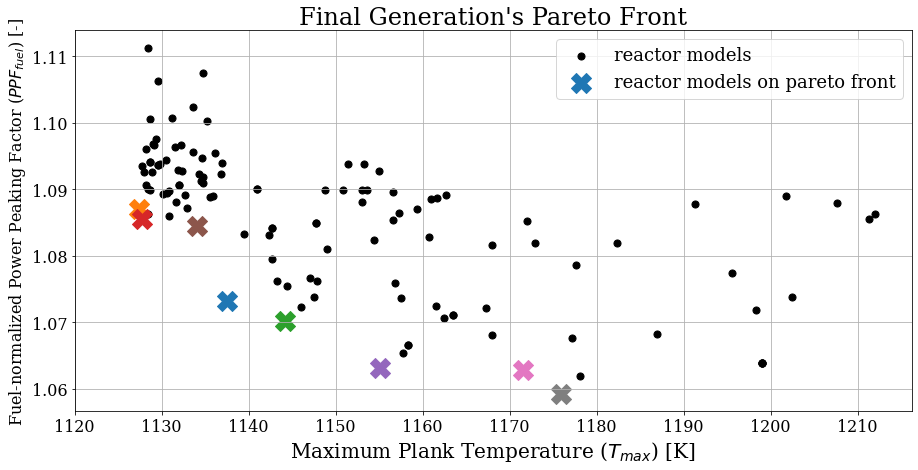
\includegraphics[width=\linewidth]{slab-obj-2-tempppf-pareto.png}
        \caption{Plot of final generation's reactor models' $T_{max}$ against 
        $PPF_{fuel}$. Crosses indicate the reactor models on the Pareto front.
        Cross colors correspond to TRISO distributions in the plot below.}
        \label{fig:slab-obj-2-tempppf-pareto} 
    \end{subfigure}
    \begin{subfigure}{\textwidth}
        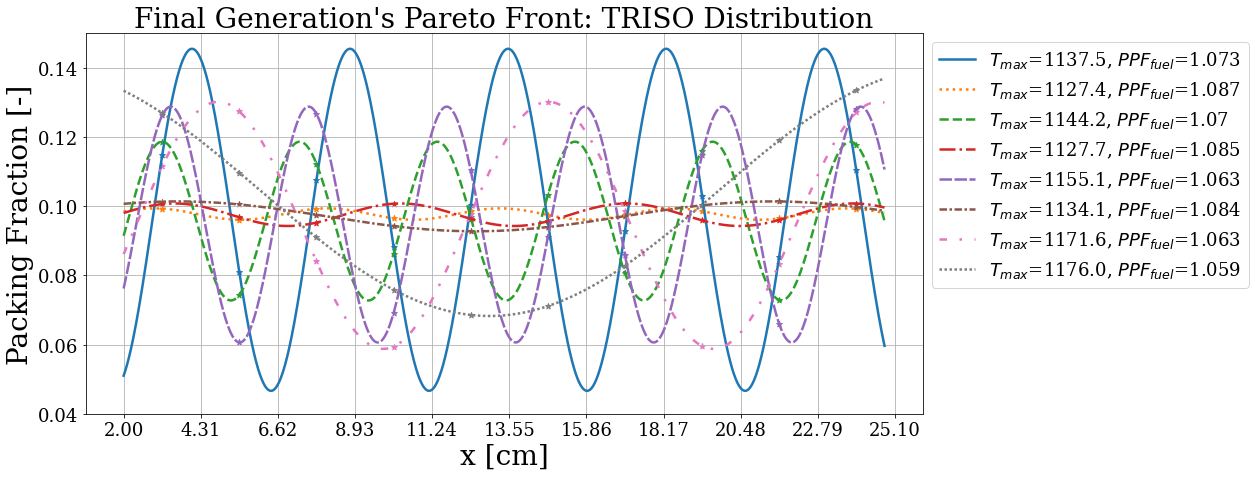
\includegraphics[width=\linewidth]{slab-obj-2-tempppf-pareto-distr.png}
        \caption{TRISO packing fraction distribution for the 8 reactor models on the 
        Pareto front.}
        \label{fig:slab-obj-2-tempppf-pareto-distr} 
    \end{subfigure}
    \caption{Simulation p-2c -- ROLLO two-objective optimization to minimize maximum 
    plank temperature ($T_{max}$) and fuel-normalized power peaking factor 
    ($PPF_{fuel}$) in the plank. 
    Input parameters varied: TRISO packing fraction distribution 
    ($\rho_{TRISO}(\vec{r})$). $PF_{total}$ = 0.0979.}
    \label{fig:slab-obj-2-tempppf}
\end{figure}
\begin{figure}[htbp!]
    \ContinuedFloat
    \begin{subfigure}{\textwidth}
        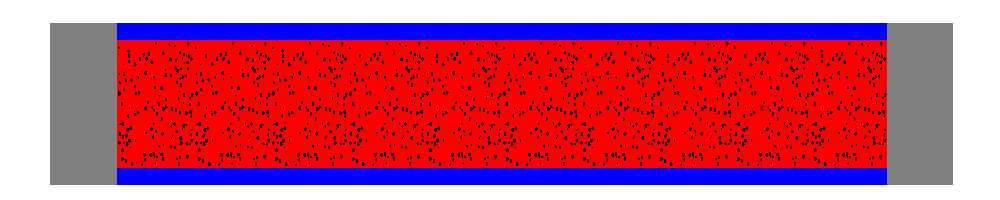
\includegraphics[width=\linewidth]{slab-obj-2-tempppf-min-temp.png}
        \caption{\gls{AHTR} plank model with most-minimized $T_{max}$
        (corresponds to the orange bolded distribution in Figure 
        \ref{fig:slab-obj-2-tempppf-pareto-distr}).}
        \label{fig:slab-obj-2-tempppf-min-temp} 
    \end{subfigure}
    \begin{subfigure}{\textwidth}
        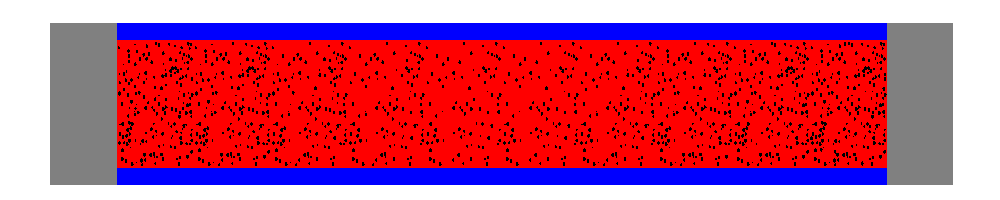
\includegraphics[width=\linewidth]{slab-obj-2-tempppf-min-ppf.png}
        \caption{\gls{AHTR} plank model with most-minimized $PPF_{fuel}$
        (corresponds to the grey bolded distribution in Figure 
        \ref{fig:slab-obj-2-tempppf-pareto-distr}).}
        \label{fig:slab-obj-2-tempppf-min-ppf} 
    \end{subfigure}
    \caption{(contd.) Simulation p-2c -- ROLLO two-objective optimization to minimize 
    maximum plank temperature ($T_{max}$) and fuel-normalized power peaking factor 
    ($PPF_{fuel}$) in the plank. 
    Input parameters varied: TRISO packing fraction distribution 
    ($\rho_{TRISO}(\vec{r})$). $PF_{total}$ = 0.0979.}
\end{figure}

In Figure \ref{fig:slab-obj-2-tempppf-pareto-distr}, the TRISO distribution with 
the most-minimized $T_{max}$ and highest $PPF_{fuel}$ (the orange distribution) 
has an almost constant packing fraction of $\sim0.10$ across the plank, with a 
slight oscillating pattern (also illustrated in Figure 
\ref{fig:slab-obj-2-tempppf-min-temp}).
This distribution follows a similar flat shape as simulation p-1b's most-minimized 
$T_{max}$ TRISO distribution (Figure \ref{fig:slab-obj-1-temp-distr}).
In Figure \ref{fig:slab-obj-2-tempppf-pareto-distr}, the TRISO distribution with 
most-minimized $PPF_{fuel}$ and highest $T_{max}$
(the grey distribution) peaks near the sides of the plank, and has a minimum point at 
the center of the plank (also illustrated in Figure \ref{fig:slab-obj-2-tempppf-min-ppf}). 
This distribution is somewhat similar to p-1c's most-minimized $PPF_{fuel}$ TRISO distribution 
(Figure \ref{fig:slab-obj-1-ppf-final}) which also has a minimum point at the center 
of the plank, but differs as its' peaks are on the fuel regions' edges instead of the 
plank's edges. 

The differences between the above cases and their single objective counterparts in 
Section \ref{sec:plank-one-obj} are due to influences from the other objectives. 

\pagebreak
\section{AHTR Plank: Three-Objective Optimization Results}
\label{sec:plank-three-obj}
In this section, I report the \gls{AHTR} one-third assembly's \gls{ROLLO} three-objective 
optimization results. 
Table \ref{tab:assem-obj-breakdown} summarized the two-objective simulations in this 
section: p-3a, and p-3b. 

\subsection{p-3a: Variation of of $PF_{total}$ and $\rho_{TRISO}(\vec{r})$}
\label{sec:p-3a}
This section reports results from the three-objective optimization simulation p-3a, all 
objectives are minimized: total fuel packing fraction ($PF_{total}$), maximum plank 
temperature ($T_{max}$) and fuel-normalized power peaking factor ($PPF_{fuel}$).  
The input parameters varied are total fuel packing fraction ($PF_{total}$) and 
TRISO packing fraction distribution ($\rho_{TRISO}(\vec{r})$). 
Table \ref{tab:simulationp3a} shows simulation p-3a's optimization problem parameters. 
\begin{table}[htbp!]
    \centering
    \onehalfspacing
    \caption{Simulation p-3a Optimization Problem Parameters}
	\label{tab:simulationp3a}
    \footnotesize
    \begin{tabular}{l|p{4cm}}
    \hline 
    \multicolumn{2}{c}{\textbf{Three Objectives: Simulation p-3a}} \\
    \hline 
    \textbf{Objectives} & Minimize $PF_{total}$ \\
    & Minimize $T_{max}$ \\
    & Minimize $PPF_{fuel}$ \\
    \hline 
    \textbf{Input parameter variations} & $0.02<PF_{total}<0.04$ \\
    & $0<a<2$ \\
    & $0<b<\frac{\pi}{2}$ \\
    & $0<c<2\pi$ \\
    \hline
    \textbf{Constraints} & $k_{eff} \geq 1.35$\\ 
    \hline 
    \textbf{Genetic algorithm parameters} & Population size: 128 \\
    & Generations: 5 \\
    \hline
    \end{tabular}
\end{table}

Table \ref{tab:p3a-hypervolume} shows the hypervolume value at each generation, 
confirming that simulation p-3a converges by generation 5. 
\begin{table}[htbp!]
    \centering
    \onehalfspacing
    \caption{Simulation p-3a hypervolume values at each generation.}
	\label{tab:p3a-hypervolume}
    \footnotesize
    \begin{tabular}{ll}
    \hline 
    \multicolumn{2}{c}{\textbf{Three Objectives: Simulation p-3a}} \\
    \multicolumn{2}{c}{Reference point: (0.06, 1260 ,1.5)} \\
    \hline 
    \textbf{Generation} & \textbf{Hypervolume value} \\
    \hline
    1 & 2.392 \\
    2 & 2.392 \\
    3 & 2.393 \\
    4 & 2.442 \\
    5 & 2.446 \\
    \hline
    \end{tabular}
\end{table}

Figure \ref{fig:slab-obj-3-3d} shows a 3D plot of the final generation's reactor models' 
$PF_{total}$ against $T_{max}$ against $PPF_{fuel}$, crosses mark the reactor models 
that fall on the Pareto front.
Figure \ref{fig:slab-obj-3-distr} shows the 14 TRISO packing fraction distributions in 
the final generation that fall on the Pareto front. 
\begin{figure}[htbp!]
    \begin{subfigure}{\textwidth}
        \centering
        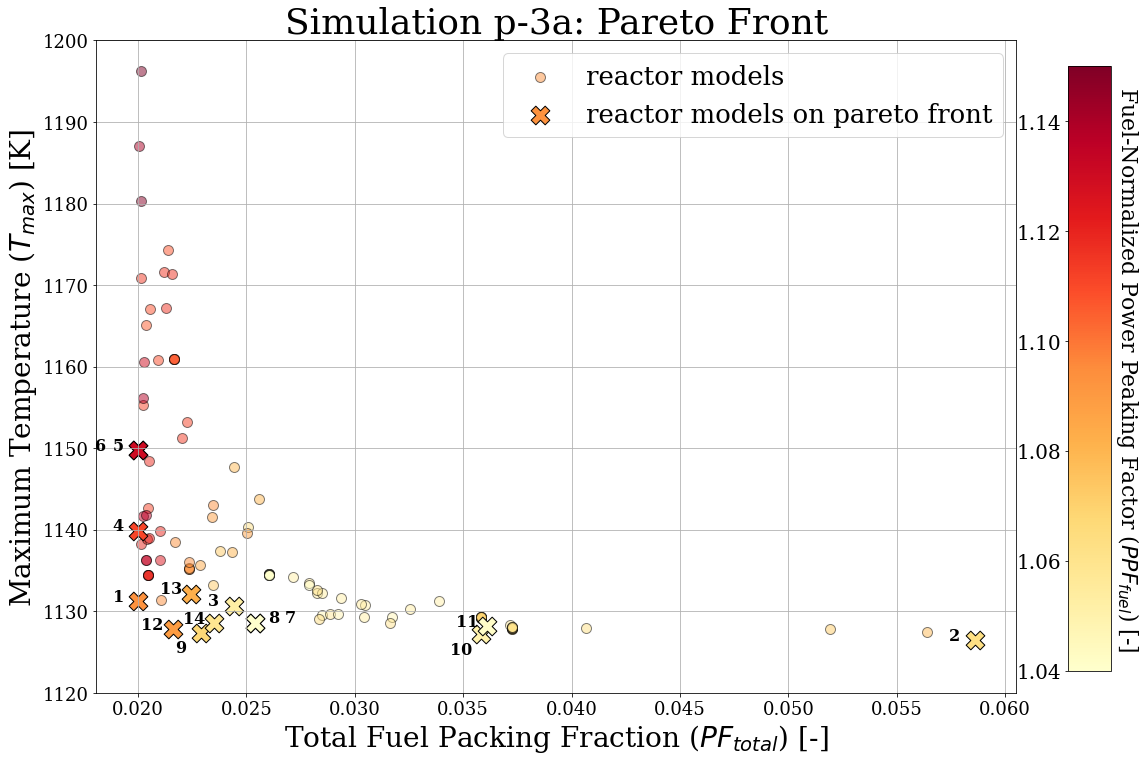
\includegraphics[width=0.7\linewidth]{slab-obj-3-3d.png}
        \caption{Plot of final generation's reactor models' $PF_{total}$ against 
        $T_{max}$ against $PPF_{fuel}$. Crosses indicate the reactor models on the 
        Pareto front. Cross colors correspond to TRISO distributions in the plot below.}
        \label{fig:slab-obj-3-3d} 
    \end{subfigure}
    \begin{subfigure}{\textwidth}
        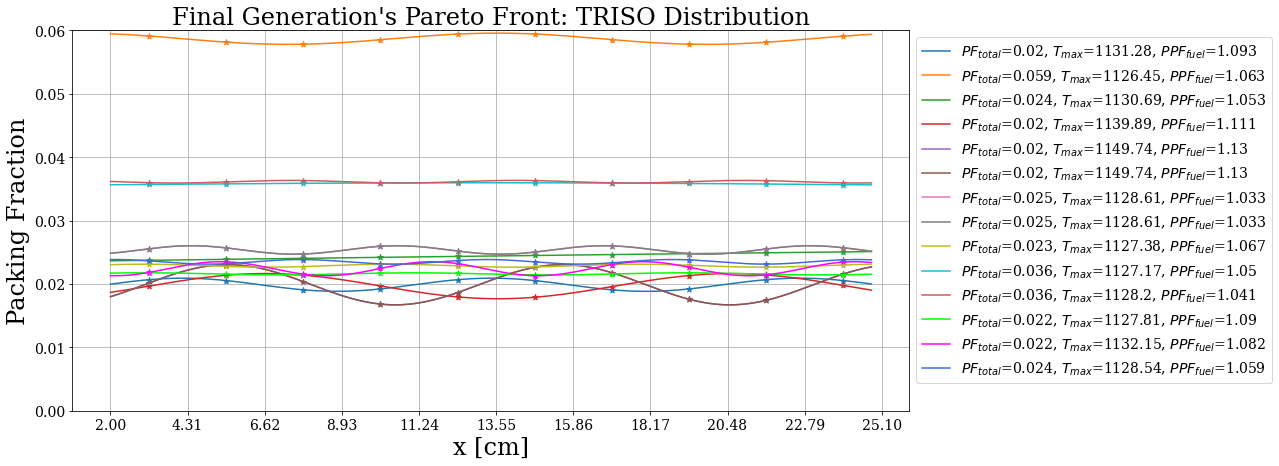
\includegraphics[width=\linewidth]{slab-obj-3-distr.png}
        \caption{TRISO packing fraction distribution for the 14 reactor models on the Pareto front.}
        \label{fig:slab-obj-3-distr} 
    \end{subfigure}
    \caption{Simulation p-3a -- ROLLO three-objective optimization to minimize total 
    fuel packing fraction ($PF_{total}$), maximum plank temperature ($T_{max}$) and 
    fuel-normalized power peaking factor ($PPF_{fuel}$) in the plank. 
    Input parameters varied: $PF_{total}$, TRISO packing fraction distribution
    ($\rho_{TRISO}(\vec{r})$).}
    \label{fig:slab-obj-3}
\end{figure}

Figure \ref{fig:slab-obj-3-3d} demonstrates that \gls{ROLLO} found 14 widely spread 
solutions in the final generation's Pareto front. 
Figure \ref{fig:slab-obj-3-distr} demonstrates that the TRISO distributions on the
Pareto front have maximum packing fraction variation of $\sim0.01$. 
Figure \ref{fig:slab-obj-3-distr-most-minimized} shows the three distributions from 
Figure \ref{fig:slab-obj-3-distr} that most-minimized each objective. 
\begin{figure}[htbp!]
    \centering
    \begin{subfigure}{\textwidth}
        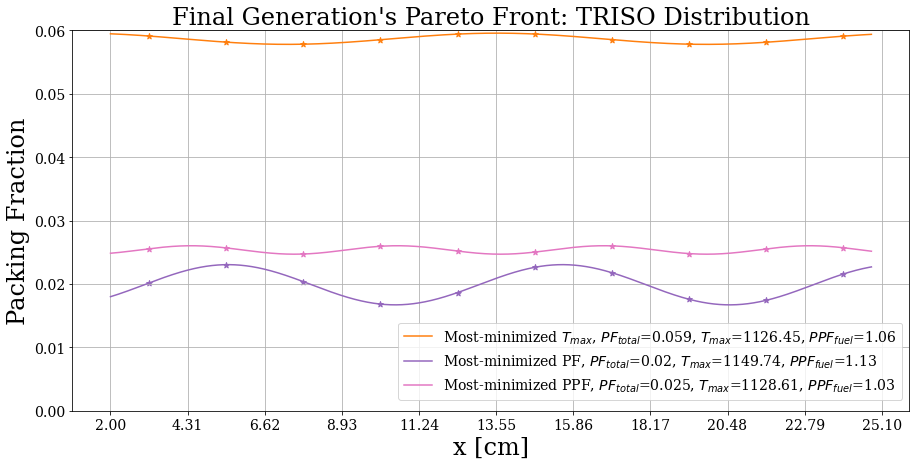
\includegraphics[width=\linewidth]{slab-obj-3-distr-most-minimized.png}
        \caption{TRISO distribution for the 3 reactor models on the Pareto front
        that most minimized each objective.}
        \label{fig:slab-obj-3-distr-most-minimized}
    \end{subfigure}
    \begin{subfigure}{0.8\textwidth}
        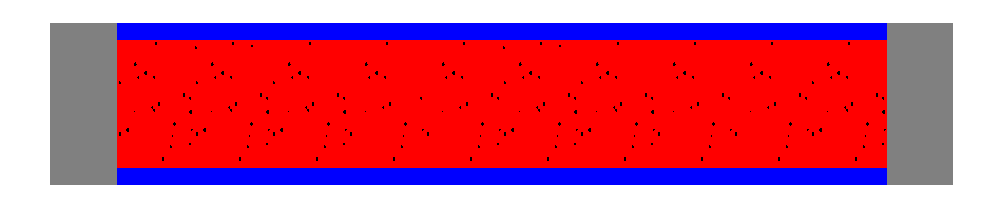
\includegraphics[width=\linewidth]{slab-obj-3-min-pf.png}
        \caption{\gls{AHTR} plank model with most-minimized $PF_{total}$ 
        (corresponds to the purple distribution in the above plot).}
        \label{fig:slab-obj-3-min-pf} 
    \end{subfigure}
    \begin{subfigure}{0.8\textwidth}
        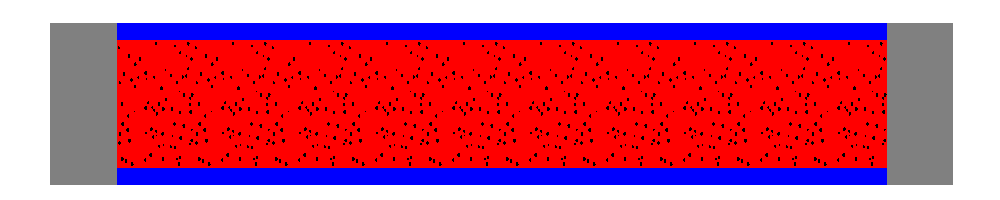
\includegraphics[width=\linewidth]{slab-obj-3-min-temp.png}
        \caption{\gls{AHTR} plank model with most-minimized $T_{max}$
        (corresponds to the orange distribution in the above plot).}
        \label{fig:slab-obj-3-min-temp} 
    \end{subfigure}
    \begin{subfigure}{0.8\textwidth}
        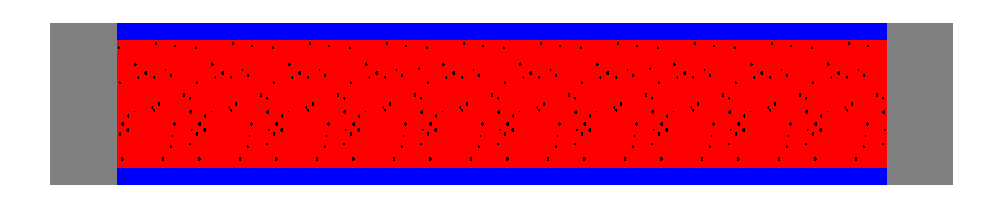
\includegraphics[width=\linewidth]{slab-obj-3-min-ppf.png}
        \caption{\gls{AHTR} plank model with most-minimized $PPF_{fuel}$
        (corresponds to the pink distribution in the above plot).}
        \label{fig:slab-obj-3-min-ppf} 
    \end{subfigure}
    \caption{AHTR plank models and TRISO distribution for the 3 reactor models on simulation 
    p-3a's Pareto front that most-minimized each objective.
    Simulation p-3a -- ROLLO three-objective optimization to minimize total fuel packing 
    fraction ($PF_{total}$), maximum plank temperature ($T_{max}$) and 
    normalized power peaking factor ($PPF_{fuel}$) in the plank. 
    Input parameters varied: $PF_{total}$, TRISO packing fraction distribution
    ($\rho_{TRISO}(\vec{r})$)}
    \label{fig:slab-obj-3-most-minimized}
\end{figure}

In Figure \ref{fig:slab-obj-3-distr-most-minimized}, the TRISO distribution with the
most-minimized $PF_{total}$ (the purple distribution) has an oscillating fuel 
packing pattern (also illustrated in Figure \ref{fig:slab-obj-3-min-pf}).
This distribution is similar to simulation p-1a's most-minimized $PF_{total}$ TRISO 
distribution (Figure \ref{fig:slab-obj-1-pf-final}) with its oscillating TRISO distribution. 
In Figure \ref{fig:slab-obj-3-distr-most-minimized}, the TRISO distribution with the 
most-minimized $T_{max}$ (the orange distribution) has mostly flat TRISO distribution 
(also illustrated in Figure \ref{fig:slab-obj-3-min-temp}). 
This distribution follows a similar distribution as simulation p-1b's most-minimized 
$T_{max}$ TRISO distribution (Figure \ref{fig:slab-obj-1-temp-final}): a mostly flat 
TRISO distribution with two small dips at the one-third and two-third points in the 
plank.
In Figure \ref{fig:slab-obj-3-distr-most-minimized}, the TRISO distribution with the
most-minimized $PPF_{fuel}$ (the pink distribution) has a 
slightly oscillating TRISO distribution (also illustrated in Figure 
\ref{fig:slab-obj-3-min-ppf}).

Most of the \gls{TRISO} distributions on the Pareto front (Figure 
\ref{fig:slab-obj-3-distr}) have a mostly flat distribution with approximately 
$\sim0.1cm$ of variation. 
The flatness is influenced by the minimize $T_{max}$ objective. 
As observed in previous sections \ref{sec:plank-1-obj-temp}, \ref{sec:p-2a}, and 
\ref{sec:p-2c}, a flat \gls{TRISO} distribution minimizes $T_{max}$ objective.
The variations in \gls{TRISO} distributions are influenced by both the minimize 
total packing fraction and minimize $PPF_{fuel}$ objectives. 
The minimize total packing fraction objective tries to minimize self shielding effects 
to enable a higher $k_{eff}$ for lower total PF. 
The fuel-normalized power peaking factor objective tries to minimize 
TRISO fuel in areas with higher flux to minimize fuel-normalized power peaking.

Section \ref{sec:plank-discussion} further discusses \gls{ROLLO}'s plank 
optimization results and significance for reactor designers.

\subsection{p-3b: Variation of $PF_{total}$, $\rho_{TRISO}(\vec{r})$, and Coolant 
Channel Shape}
This section reports results from the three-objective optimization simulation p-3b, 
all objectives are minimized: total fuel packing fraction ($PF_{total}$), maximum plank 
temperature ($T_{max}$) and fuel-normalized power peaking factor ($PPF_{fuel}$).  
The input parameters varied are total fuel packing fraction ($PF_{total}$), 
TRISO packing fraction distribution ($\rho_{TRISO}(\vec{r})$), and coolant channel 
shape.  
Table \ref{tab:simulationp3b} shows simulation p-3b's optimization problem parameters. 
\begin{table}[htbp!]
    \centering
    \onehalfspacing
    \caption{Simulation p-3b Optimization Problem Parameters}
	\label{tab:simulationp3b}
    \footnotesize
    \begin{tabular}{l|p{4cm}}
    \hline 
    \multicolumn{2}{c}{\textbf{Three Objectives: Simulation p-3b}} \\
    \hline 
    \textbf{Objectives} & Minimize $PF_{total}$ \\
    & Minimize $T_{max}$ \\
    & Minimize $PPF_{fuel}$ \\
    \hline 
    \textbf{Input parameter variations} & $0.02<PF_{total}<0.04$ \\
    & $0<a<2$ \\
    & $0<b<\frac{\pi}{2}$ \\
    & $0<c<2\pi$ \\
    & $0.05<r_{top}<0.35$ \\
    & $0.05<r_{bot}<0.35$ \\
    \hline
    \textbf{Constraints} & $k_{eff} \geq 1.35$\\ 
    \hline 
    \textbf{Genetic algorithm parameters} & Population size: 128 \\
    & Generations: 8 \\
    \hline
    \end{tabular}
\end{table}

Table \ref{tab:p3b-hypervolume} shows the hypervolume value at each generation, 
confirming that simulation p-3b converges by generation 8. 
\begin{table}[htbp!]
    \centering
    \onehalfspacing
    \caption{Simulation p-3b hypervolume values at each generation.}
	\label{tab:p3b-hypervolume}
    \footnotesize
    \begin{tabular}{ll}
    \hline 
    \multicolumn{2}{c}{\textbf{Three Objectives: Simulation p-3b}} \\
    \multicolumn{2}{c}{Reference point: (0.06, 1260 ,1.5)} \\
    \hline 
    \textbf{Generation} & \textbf{Hypervolume value} \\
    \hline
    1 & 1.985 \\
    2 & 2.119 \\
    3 & 2.158 \\
    4 & 2.251\\
    5 & 2.262 \\
    6 & 2.280 \\
    7 & 2.310 \\
    8 & 2.313 \\
    \hline
    \end{tabular}
\end{table}

Figure \ref{fig:slab-obj-3-3d-all} shows a 3D plot of the final generation's reactor 
models' $PF_{total}$ against $T_{max}$ against $PPF_{fuel}$, crosses mark the 
reactor models that fall on the Pareto front.
Figure \ref{fig:slab-obj-3-distr-all} shows the 21 TRISO distributions and their
total radius $(r_{top}, r_{bot})$ in the final generation that fall on the Pareto 
front. 
\begin{figure}[htbp!]
    \begin{subfigure}{\textwidth}
        \centering
        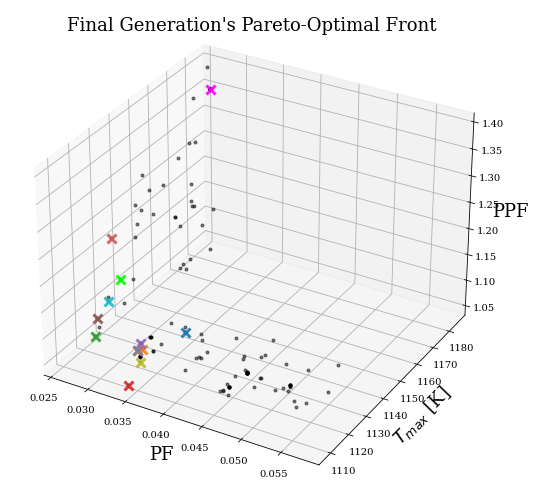
\includegraphics[width=0.7\linewidth]{slab-obj-3-3d-all.png}
        \caption{Plot of final generation's reactor models' $PF_{total}$ against 
        $T_{max}$ against $PPF_{fuel}$. Crosses indicate the reactor models on the 
        Pareto front. Cross colors correspond to TRISO distributions in the plot below.}
        \label{fig:slab-obj-3-3d-all} 
    \end{subfigure}
    \begin{subfigure}{\textwidth}
        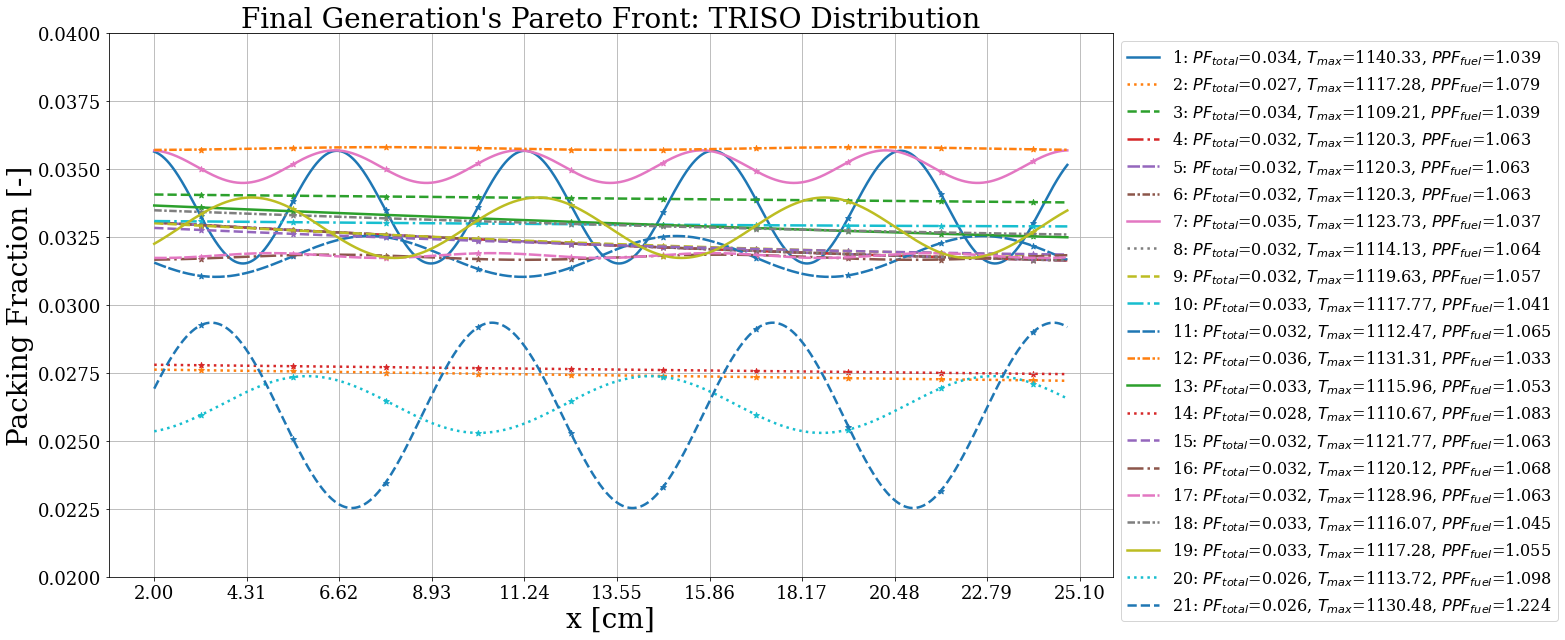
\includegraphics[width=\linewidth]{slab-obj-3-distr-all.png}
        \caption{TRISO distribution for the 21 reactor models on the Pareto front.}
        \label{fig:slab-obj-3-distr-all} 
    \end{subfigure}
    \caption{Simulation p-3b -- ROLLO three-objective optimization to minimize total 
    fuel packing fraction ($PF_{total}$), maximum plank temperature ($T_{max}$), and 
    fuel-normalized power peaking factor ($PPF_{fuel}$) in the plank. 
    Input parameters varied: total fuel packing fraction $PF_{total}$, 
    TRISO packing fraction distribution ($\rho_{TRISO}(\vec{r})$), 
    coolant channel shape $(r_{top}, r_{bot})$.}
    \label{fig:slab-obj-3-all}
\end{figure}

Figure \ref{fig:slab-obj-3-3d-all} demonstrates that \gls{ROLLO} found 21 widely spread 
solutions in the final generation's Pareto front. 
Figure \ref{fig:slab-obj-3-distr-most-minimized-distr-all} shows the three distributions 
from Figure \ref{fig:slab-obj-3-distr-all} that most-minimized each objective. 
Figures \ref{fig:slab-obj-3-all-min-pf}, \ref{fig:slab-obj-3-all-min-temp}, and 
\ref{fig:slab-obj-3-all-min-ppf} show the \gls{AHTR} plank's TRISO distribution and 
coolant channel shape for most-minimized cases. 
\begin{figure}[htbp!]
    \begin{subfigure}{\textwidth}
        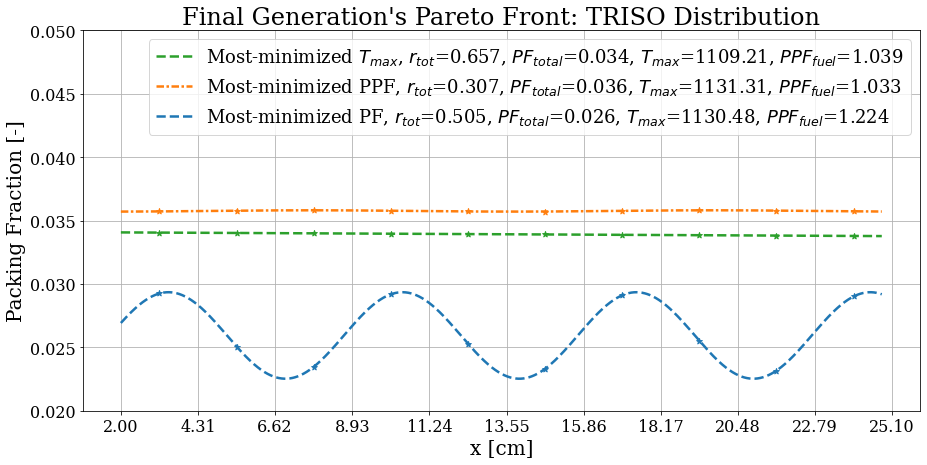
\includegraphics[width=\linewidth]{slab-obj-3-distr-most-minimized-all.png}
        \caption{TRISO distribution for the 3 reactor models on the Pareto 
        front that most minimized each objective.}
        \label{fig:slab-obj-3-distr-most-minimized-distr-all}
    \end{subfigure}
    \begin{subfigure}{\textwidth}
        
\includegraphics[width=\linewidth]{slab-obj-3-all-min-pf.png}
        \caption{TRISO distribution and coolant channel shape that most-minimized 
        $PF_{total}$ (corresponds to the red distribution in the above plot).}
        \label{fig:slab-obj-3-all-min-pf}
    \end{subfigure}
    \begin{subfigure}{\textwidth}
        
\includegraphics[width=\linewidth]{slab-obj-3-all-min-tempppf.png}
        \caption{TRISO distribution and coolant channel shape that most minimized 
        $T_{max}$ (corresponds to the pink distribution in the above plot).}
        \label{fig:slab-obj-3-all-min-temp}
    \end{subfigure}
    \begin{subfigure}{\textwidth}
        
\includegraphics[width=\linewidth]{slab-obj-3-all-min-tempppf.png}
        \caption{TRISO distribution and coolant channel shape that most minimized 
        $PPF_{fuel}$ (corresponds to the pink distribution in the above plot).}
        \label{fig:slab-obj-3-all-min-ppf}
    \end{subfigure}
    \caption{AHTR models and TRISO distribution for the 3 reactor models on simulation 
    p-3b -- ROLLO three-objective optimization to minimize total 
    fuel packing fraction ($PF_{total}$), maximum plank temperature ($T_{max}$), and 
    fuel-normalized power peaking factor ($PPF_{fuel}$) in the plank. 
    Input parameters varied: total fuel packing fraction $PF_{total}$, 
    TRISO packing fraction distribution ($\rho_{TRISO}(\vec{r})$), 
    coolant channel shape $(r_{top}, r_{bot})$.}
    \label{fig:slab-obj-3-distr-most-minimized-all}
\end{figure}

In Figure \ref{fig:slab-obj-3-distr-most-minimized-distr-all}, the \gls{AHTR} plank model 
with the most-minimized $PF_{total}$ (the pink distribution) has a oscillating fuel 
packing pattern with approximately $\sim0.2cm$ of variation and total coolant channel radius 
of 0.399cm (illustrated in Figure \ref{fig:slab-obj-3-all-min-pf}).
In Figure \ref{fig:slab-obj-3-distr-most-minimized-distr-all}, the \gls{AHTR} plank model with 
the most-minimized $T_{max}$ and $PPF_{fuel}$ (the red distribution) 
has a flat TRISO distribution and total coolant channel radius of 0.657cm 
(illustrated in Figure \ref{fig:slab-obj-3-all-min-tempppf}). 

Similar to simulation p-3a (Section \ref{sec:p-3a}), most of the \gls{TRISO} distributions 
on the Pareto front have a mostly flat distribution with maximum $\sim0.1cm$ of 
variation. 
The flatness is influenced by the minimize $T_{max}$ objective. 
As observed in previous sections \ref{sec:plank-1-obj-temp}, \ref{sec:p-2a}, and 
\ref{sec:p-2c}, a flat \gls{TRISO} distribution minimizes $T_{max}$ objective.
The variations in \gls{TRISO} distributions are influenced by both the minimize 
$PF_{total}$ and minimize $PPF_{fuel}$ objectives. 
The minimize total packing fraction objective tries to minimize self shielding effects 
to enable a higher $k_{eff}$ for lower total PF. 
The minimize fuel-normalized power peaking factor objective tries to minimize 
TRISO distribution in areas with higher flux to minimize fuel-normalized power peaking.
% talk about coolant channel shape influences T_max. but not as much 
% the other objectives are not impacted by coolant channel shape. 

Section \ref{sec:plank-discussion} further discusses \gls{ROLLO}'s plank 
optimization results and significance for reactor designers.

\pagebreak
\section{AHTR Plank: Computational Cost Summary}
\label{sec:plank-compute-cost}
Optimization simulations are run on the BlueWaters supercomputer \cite{ncsa_about_2017} and
the Theta supercomputer at the Argonne Leadership Computing Facility under the Director's 
Discretionary Allocation Program \cite{noauthor_argonne_2022}. 
Each BlueWaters compute node has 32 processor cores with a nominal clock speed of 3.2GHz
\cite{ncsa_about_2017}, and each Theta compute node has 64 processor cores with a nominal 
clock speed of 1.5GHz \cite{noauthor_argonne_2022}.  

Each optimization simulation takes a different amount of node-hours to run due to 
differences in simulation software, tallies and intermediate steps required. 
Table \ref{tab:plank-compute-cost} reports the computational cost for each optimization 
simulation. 
Table \ref{tab:slab-obj-breakdown} detailed the simulation parameters.
\begin{table}[htbp!]
    \centering
    \onehalfspacing
    \caption{Computational cost of \acrfull{ROLLO} simulations for optimizing \acrfull{AHTR}
    plank. BW: BlueWaters Supercomputer, Theta: Theta supercomputer.}
	\label{tab:plank-compute-cost}
    \footnotesize
    \begin{tabular}{p{1.4cm}|p{1cm}lp{4cm}lp{4cm}}
    \hline 
    \textbf{Num of Objs} & \textbf{Sim} & \textbf{Machine} & \textbf{Compute cost per gen [node-hours]} &\textbf{gens} & \textbf{Total compute cost [node-hours]} \\
    \hline
    \multirow{6}{2cm}{1} 
    & p-1a & BW & 23.9 & 10 & 238.7 \\
    & p-1b & BW & 96.0 & 10 & 959.7 \\
    & p-1c & BW & 65.9 & 10 & 658.6 \\
    & p-1d & Theta & 49.6 & 3 & 148.7 \\
    & p-1e & Theta & 71.4 & 4 & 285.6 \\
    & p-1f & Theta & 46.4 & 5 & 231.8 \\
    \hline
    \multirow{3}{2cm}{2}
    & p-2a & Theta & 132.2 & 2 & 264.5 \\
    & p-2b & Theta & 66.3 & 3 & 198.9 \\
    & p-2c & Theta & 167.1 & 3 & 501.2 \\
    \hline
    \multirow{2}{2cm}{3}
    & p-3a & Theta & 92.9 & 5 & 464.5 \\
    & p-3b & Theta & 181.2 & 5 & 906.2 \\
    \hline
    \end{tabular}
\end{table}
